\chapter{Périmètres et aires} \label{M13}

\begin{figure}[h]
   \centering
      \DeclareFixedFont{\ps}{U}{psy}{m}{n}{7cm}
      \begin{pspicture}(-3,-3)(3,3)
         \rput(0,-2){\pscharpath[linecolor=B2,fillstyle=solid,fillcolor=B2,opacity=0.5]{\rput[b](0,0){\ps p}}}
         \pstextpath{
            \pscustom[linestyle=none]{%
               \parametricplot[plotpoints=500]{0}{1350}{t cos t 500 div mul t sin t 500 div mul}
               \psline(!51 cos 51 600 div mul 600 add 51 sin 3510 600 div mul)}}
               {3,141 592 653 589 793 238 462 643 383 279 502 884 197 169 399 375 105 820 974 944 592 307 816 406 286 208 998 628 034 825 342 117 067 982 148 086 513 282 306 647 093 844 609 550 582 231 725 359 408 128 481 117 450 284 102 701 938 521 105 559 644 622 948 954 930\dots}
      \end{pspicture}
\end{figure}

\begin{prerequis}[Un peu d'histoire]
   Parmi les nombres qui permettent de mesurer des longueurs ou des aires, il en est un indispensable pour tout ce qui concerne les cercles et les disques : le nombre $\pi$. \\
   La quadrature du cercle est un problème classique de mathématiques apparaissant en géométrie. Il fait partie des trois grands problèmes de l'Antiquité, avec la trisection de l'angle et la duplication du cube. Il consiste à construire un carré de même aire qu'un disque donné à l'aide d'une règle et d'un compas. La quadrature du cercle nécessite la construction à la règle et au compas de la racine carrée du nombre $\pi$, ce qui est impossible. Ce problème mathématique est celui qui a résisté le plus longtemps aux mathématiciens, qui ont mis plus de trois millénaires à étudier le problème, reconnu comme insoluble par Ferdinand von Lindemann en 1882. \\
   $\pi$ est un nombre, au même titre que 2 ou 100 ou 6,538, sauf que son écriture décimale est infinie. Il désigne le rapport du périmètre d'un cercle par son diamètre. Là aussi, de nombreux mathématiciens ont tenté de découvrir la valeur la plus fiable de $\pi$ par des méthodes diverses. L'une d'elles, celle d'Archimède (250 avant J.-C.), consistait à encadrer l'aire d'un disque de rayon 1 (donc $\pi$) par l'aire d'un polygone régulier inscrit dans ce disque, et par l'aire d'un polygone régulier exinscrit, dont les aires sont plus simples à calculer.
\end{prerequis}
   
   
\cours

%%%%%%%%%%%%%%%%%%
\section{Repères historiques} %%% I
%%%%%%%%%%%%%%%%%%
\label{un}

En 1795, il existe en France plus de sept cents unités de mesure différentes qui varient d'une ville à l'autre. Beaucoup sont empruntées à la morphologie humaine : la paume, la palme, l'empan, le pied, la coudée, le pas, la brasse\dots{} 
\begin{center}
   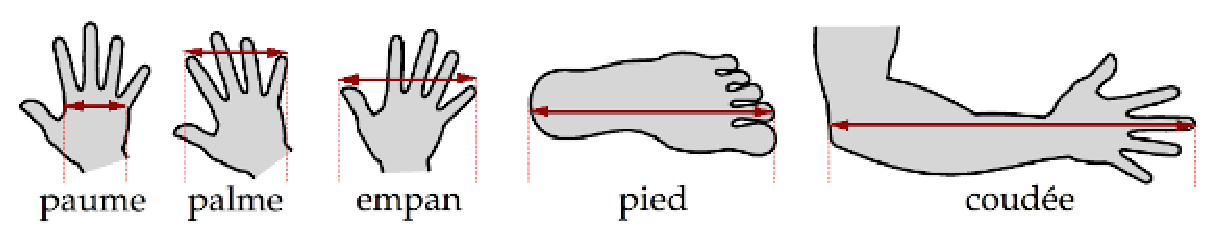
\includegraphics[width=10cm]{Grandeurs_mesures/Images/M13_cours_humain}
\end{center}
Source d'erreurs et de fraudes lors des transactions commerciales, cette situation porte préjudice au développement des sciences. Politiques et scientifiques vont tenter de réformer cet état de fait. Leur idée est d'assurer l'invariabilité des mesures en les rapportant à un étalon emprunté à un phénomène naturel, un étalon universel qui permettrait l'adhésion de toutes les nations étrangères. Il est alors décidé que le mètre (du grec \textit{metron}, mesure) serait défini comme la longueur de la dix-millionième partie du quart du méridien terrestre \footnote{À l’époque, un méridien (astronomique) est un grand cercle passant par les pôles. Donc pour la Terre autour de 40 000 km, le 10 millionième du quart du méridien correspond bien à 1 m. Actuellement, on définit le méridien géographique comme un demi grand cercle.}. 

\begin{minipage}{3.25cm}
   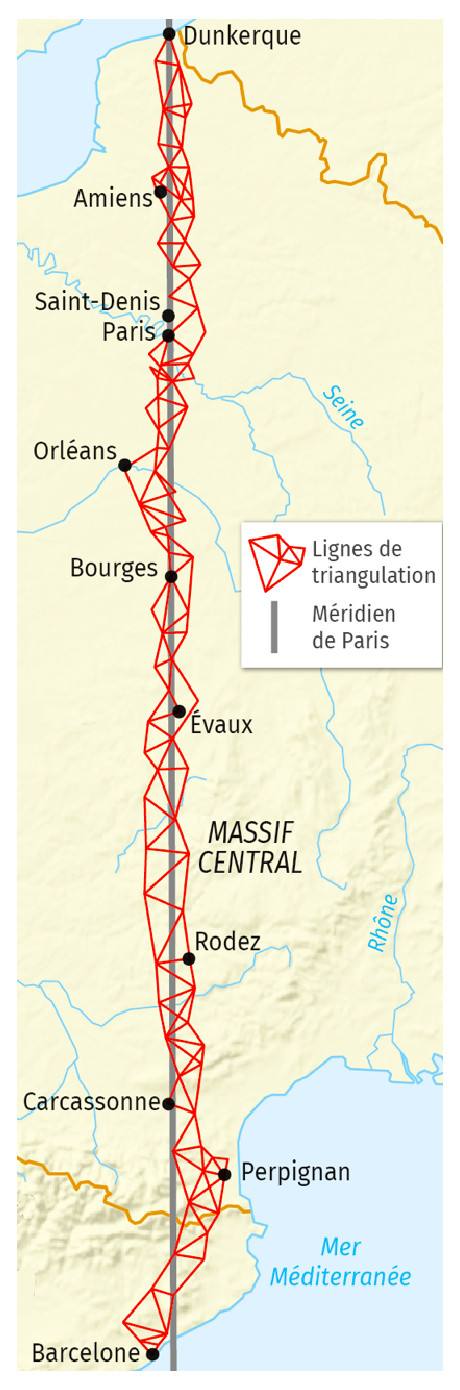
\includegraphics[width=2.8cm]{Grandeurs_mesures/Images/M13_cours_meridien}
\end{minipage}
\begin{minipage}{13.45cm}
   Ce sont les géodésiens Pierre-François \textbf{Mechain} (1744-1804) et Jean-Baptiste \textbf{Delambre} (1747-1822) qui vont se charger des opérations de triangulation permettant de donner une mesure fiable au mètre : ils devront mesurer la distance entre Dunkerque à Barcelone (situés sur le méridien de Paris, et distants de 10\degre{} de latitude). Ces travaux prennent près de sept ans et il faut plus de cent triangles pour jalonner l'arc du méridien. Sur ce parcours, nos deux hommes connaissent bien des mésaventures : arrestations, révocations temporaires, ou encore endommagement et destruction de leurs ouvrages géodésiques\footnotemark[2]. C'est ainsi que, le 26 mars 1791, nait le mètre. \\ [2mm] 
   L'unité de mesure de base étant déterminée, il suffit désormais d'établir toutes les autres unités de mesure qui en découlent : le mètre carré et le mètre cube, le litre, le gramme\dots{} \\
   Le {\bf système métrique décimal} est institué le 7 avril 1795. Il s'agit d'un bouleversement majeur des pratiques humaines. De plus, la décimalisation introduit une véritable révolution dans la conversion des différentes mesures : tout passage d'un multiple à un sous-multiple, et vice versa s'opère par simple glissement des chiffres d'un nombre dans le tableau de numération. Le {\bf système international d'unité} (SI), son successeur, voit le jour officiellement en 1960.
\end{minipage}
\footnotetext[2]{Le reportage \og \href{https://www.dailymotion.com/video/x1ns2j0}{Un mètre pour mesurer le monde} \fg{} rend compte de cette épopée.}

Au départ, le système est composé de trois unités : le {\bf mètre}, le {\bf kilogramme} et la {\bf seconde}. Mais au fur et à mesure que les sciences progressent, de nouvelles unités apparaissent : l'{\bf ampère} pour l'intensité électrique en 1946, le {\bf kelvin} pour la température et la {\bf candela} pour l'intensité lumineuse en 1954. Enfin, la {\bf mole} pour la quantité de matière fait son apparition en 1971. À ces 7 unités du SI s'ajoute le radian : unité sans dimension permettant de mesurer un angle. On peut alors en théorie se contenter de ces unités pour exprimer toutes les grandeurs physiques par combinaisons. \\
Ces unités doivent s’adapter aux progrès technologiques, et donc,  leurs définitions évoluent pour permettre des mesures avec des précisions de plus en plus fines, tout en assurant une comparabilité fiable à long terme et une uniformité en tout lieu. C'est ainsi que, depuis 2018, toutes les unités du SI sont définies par rapport à des contantes de la nature. Les seuls pays à ne pas avoir adopté, de manière officielle, le système métrique sont le Liberia, la Birmanie et les États-Unis.

\begin{minipage}{7cm}
   \begin{pspicture}(-3.5,-4)(3.5,2.5)
         \pscircle*[linecolor=gray](0,0){2.5}
         \pswedge*[linecolor=orange](0,0){2}{13}{65}
         \rput(1.25;38){\large\white m}
         \pstextpath[c]{\psarcn[linestyle=none](0,0){3}{65}{13}}{longueur}
         \pswedge*[linecolor=red](0,0){2}{65}{116}
         \rput(1.25;88){\large\white kg}
         \pstextpath[c]{\psarcn[linestyle=none](0,0){3}{116}{65}}{masse}
         \pswedge*[linecolor=magenta](0,0){2}{116}{167}
         \rput(1.25;141){\large\white s}
         \pstextpath[c]{\psarcn[linestyle=none](0,0){3}{167}{116}}{durée}
         \pswedge*[linecolor=violet](0,0){2}{167}{218}
         \rput(1.25;189){\large\white A}
         \pstextpath[c]{\psarc[linestyle=none](0,0){3}{167}{218}}{intensité du}
         \pstextpath[c]{\psarc[linestyle=none](0,0){3.5}{167}{218}}{courant électrique}
         \pswedge*[linecolor=blue](0,0){2}{218}{270}
         \rput(1.25;241){\large\white K}
         \pstextpath[c]{\psarc[linestyle=none](0,0){3}{218}{270}}{température}
         \pswedge*[linecolor=cyan](0,0){2}{270}{321}
         \rput(1.25;293){\large\white cd}
         \pstextpath[c]{\psarc[linestyle=none](0,0){3}{270}{321}}{intensité }
         \pstextpath[c]{\psarc[linestyle=none](0,0){3.5}{270}{321}}{lumineuse}
         \pswedge*[linecolor=green](0,0){2}{321}{13}
         \rput(1.25;347){\large\white mol}
         \pstextpath[c]{\psarc[linestyle=none](0,0){3}{321}{13}}{quantité}
         \pstextpath[c]{\psarc[linestyle=none](0,0){3.5}{321}{13}}{de matière}
      \end{pspicture}
\end{minipage}
\begin{minipage}{11cm}
   \begin{remarques}
      \begin{itemize}
         \item Les symboles des unités sont exprimés en minuscules, sauf s'ils sont dérivés de noms propres.
         \item Le symbole L fut adopté en 1979, comme alternative pour éviter le risque de confusion entre la lettre l et le chiffre 1.
         \item Le quotient de deux unités s'écrit avec une barre oblique, horizontale ou avec un exposant négatif : \\ [1mm]
         par exemple \quad m/s ; $\dfrac{\text{m}}{\text{s}}$ ou m.s$^{-1}$. \\ [5mm]
      \end{itemize}
   \end{remarques}
\end{minipage}

Voici par exemple un tableau dressé conformément à la loi du 11 juillet et au décret du 28 juillet 1903 sur les poids et mesures : les six unités principales sont alors le mètre pour les longueurs, l'are pour les mesures agraires, la stère pour le bois, le litre pour les mesures de capacité, le kilogramme pour les poids et le franc pour la monnaie. Le tableau montre des instruments usuels de mesures ainsi que leurs sous-mesures et sur-mesures.
\begin{center}
   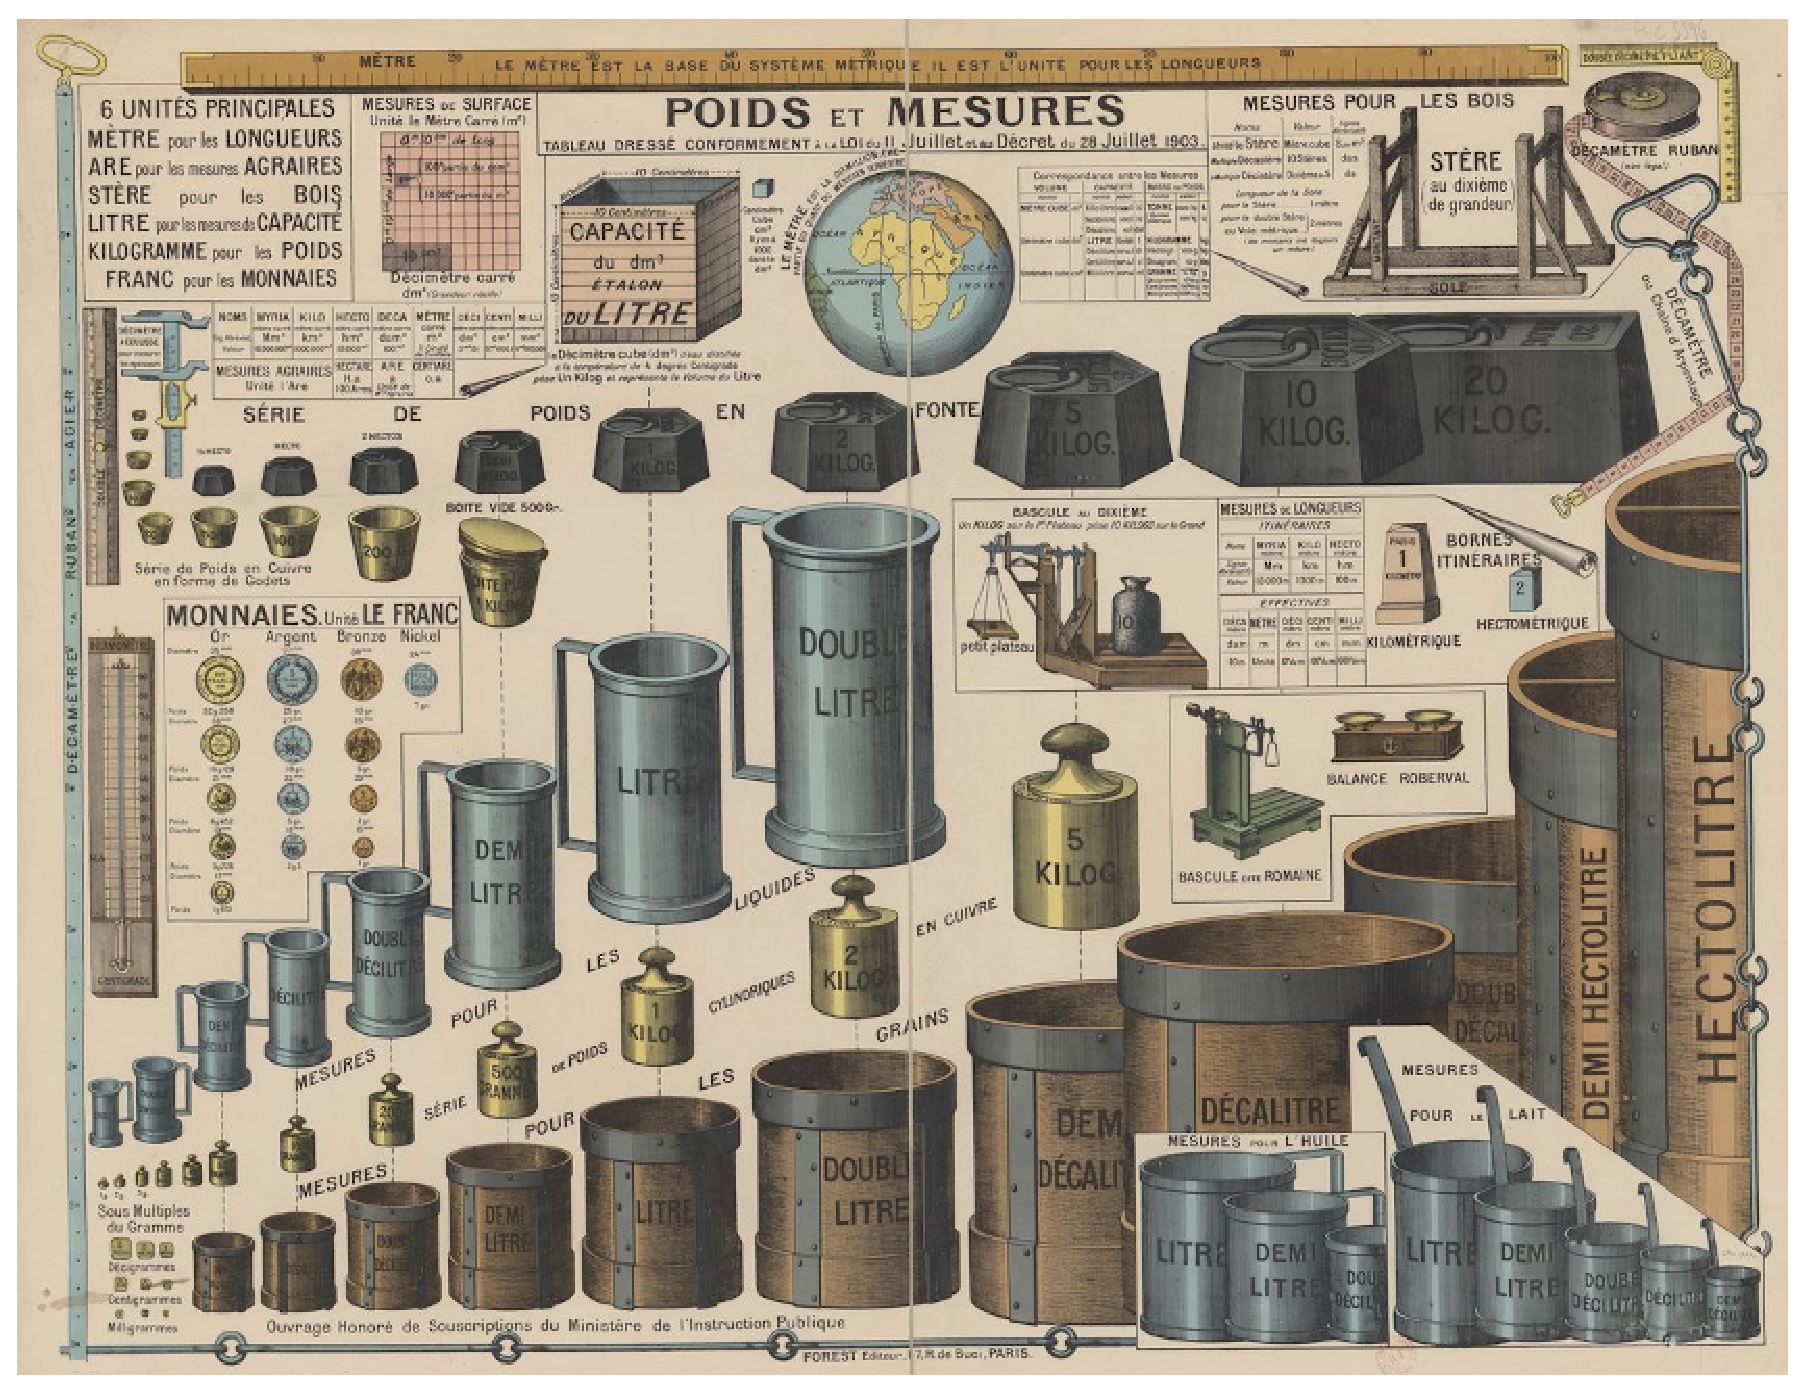
\includegraphics[width=16.5cm]{Grandeurs_mesures/Images/M13_M14_cours_intro_poids_et_mesures}
\end{center}    
{\it Tableau visible en détails sur \href{https://gallica.bnf.fr/ark:/12148/btv1b53066549q#}{Gallica, bibliothèque numérique de la Bibliothèque nationale de France.}}



%%%%%%%%%%%%%%%%%%
\section{Repères théoriques} %%% 2
%%%%%%%%%%%%%%%%%%
\label{deux}

%%%%%%%%%%%%%%%%%%%
\subsection{Grandeur VS mesure} % 2.A

Dans le VIM (vocabulaire international de métrologie), on trouve la définition suivante d'une {\bf grandeur} :
\begin{quote}
   {\it Propriété d'un phénomène, d'un corps ou d'une substance, que l'on peut exprimer quantitativement sous forme d'un nombre et d'une référence.}
\end{quote}
{\bf Mesurer} une grandeur c'est chercher combien de fois elle renferme une autre grandeur de même espèce prise pour unité de mesure. \smallskip
   
{\renewcommand{\StringDOCUMENTATION}{Une grandeur peut être}
\begin{documentation}
   \begin{itemize}
      \item \textbf{repérable} : c'est une grandeur pour laquelle on peut définir une relation d'ordre qui permet de comparer et d'ordonner des objets selon cette grandeur ;
      \item \textbf{mesurable} : il faut de plus que la grandeur de deux objets réunis soit égale à la somme des grandeurs de chaque objet et que la grandeur d’un certain nombre $n$ d’objets identiques réunis soit égale à $n$ fois la grandeur de l’objet. \\ [-8mm]
   \end{itemize}
\end{documentation}

{\psset{yunit=0.8}
\begin{pspicture}(-1.5,0)(14,7)
   \psframe[framearc=0.5,linecolor=A1](3.5,0.5)(10,5.5)
   \rput(6.5,5.2){\textcolor{A1}{grandeurs mesurables}}
   \psline[linecolor=A1](3.65,4.9)(9.85,4.9)
   \psframe[framearc=0.5,linecolor=B1](0.5,0)(10.5,6.5)
   \rput(5.5,6.2){\textcolor{B1}{grandeurs repérables}}
   \psline[linecolor=B1](0.8,5.9)(10.2,5.9)
   \rput(5,3){longueur}
   \rput(6,1){aire}
   \rput(6,4.5){volume}
   \rput(8,1.5){capacité}
   \rput(9,4){durée}
   \rput(2,4){horaires}
   \rput(12,4.5){beauté}
   \rput(12,2.5){gentillesse}
   \rput(2,2.5){température}
   \rput(7,3.7){masse}
   \rput(8,2.7){prix}
   \rput(5,2){angle}
   \rput(2,1){date}
\end{pspicture}}

\begin{exemple*1}
   La température est une grandeur repérable : on peut la repérer à l'aide d'un thermomètre. Par contre, si on ouvre une fenêtre sur l'extérieur, la température obtenue n'est pas égale à la somme des températures ; et s'il fait 5°C à l’extérieur, on ne peut pas donner de sens à l’expression \og demain il fera trois fois plus froid \fg, ce n'est donc pas une grandeur mesurable. \\ [-4mm]
\end{exemple*1}

\bigskip

En mathématiques, on utilise des nombres qui sont les nombres habituels, et les \textbf{nombres-de} qui sont des nombres accompagnés d'une unité. Ces derniers sont utilisés pour les grandeurs mesurables. On ne peut pas écrire une égalité entre nombre et nombre-de. 
   
\begin{exemple*1}
   Une écriture du type : AB + BC = 12 + 3 = \um{15} n'a aucun sens mathématique. \\
    On écrira plutôt AB + BC = \um{12} + \um{3} = \um{15}, \\
    ou alors : avec des mesures en \um{}, on a AB + BC = 12 + 3 = 15.
\end{exemple*1}

\bigskip

L'avantage d'une écriture avec les unités est aussi de vérifier la cohérence des calculs et des unités et d'effectuer des conversions si besoin.

\begin{exemple*1}
   $\udl{12}+\ul{3} \neq 15 ?$ mais $\udl{12}+\ul{3}=\udl{12}+\udl{30} =\udl{42} =\ul{4,2}$. 
\end{exemple*1}


%%%%%%%%%%%%%%%%%%%
\subsection{Longueurs et périmètres} %2.B

L'unité du SI qui permet de mesurer une longueur est le mètre (m),  et toutes les unités qui en découlent. Pour désigner les multiples ou les subdivisions des mesures, on utilise les préfixes :
\begin{center}
{\hautab{1.3}
   \begin{CLtableau}{0.8\linewidth}{8}{p{3cm}}
      \hline
      Préfixe & kilo & hecto & déca & & déci & centi & milli \\
      \hline
      Signification & $1000$ & $100$ & $10$ & $1$ & $\dfrac{1}{{\white_1}10{\white_1}}$ &
      $\dfrac{1}{{\white_1}100{\white_1}}$ & $\dfrac{1}{{\white_1}1000{\white_1}}$ \\
      \hline
      Abréviation & k & h & da & & d & c & m \\
      \hline
      Unité de longueur & km & hm & dam & m & dm & cm & mm \\
      \hline
      Exemple & & $9$ & $7$ & $3$ & $2$ & $1$ & $0$ \\
      \hline
   \end{CLtableau}}
\end{center}

Ainsi, pour convertir d'une unité à l'autre, on multiplie ou on divise par $10$, $100$, $1\,000$, \dots

\begin{exemple*1}
   $\um{973,21} =\udm{9732,1} =\uhm{9,7321} =\umm{973210}$. 
\end{exemple*1}

\begin{definition}[Périmètre et circonférence]
   Le \textbf{périmètre} d'une figure est la mesure du contour de cette figure. \\
   Pour un disque, on parle aussi de {\bf circonférence}.
\end{definition}

\begin{propriete}[Calcul d'un périmètre et d'une circonférence]
   Le {\bf périmètre} d'un polygone s'obtient en additionnant la mesure de chacun de ses segments. \\
   La {\bf circonférence} d'un disque se rayon $r$ se calcule grâce à la formule : $2\pi\,r$.
\end{propriete}

\medskip
La circonférence d'un disque de rayon $r$ est donc proportionnelle à son diamètre $d$, on peut aussi écrire $p =\pi\times d$ où $\pi \simeq 3,141\,592\,653\,589\,793\,238\,462\,643\,383\,279\,50\dots{} \simeq 3,14$. \medskip

\begin{Ltableau}{0.97\linewidth}{4}{C{4}|p{2.6cm}|C{3.5}|p{4.5cm}}
   \hline 
   Figure plane & Mesure & Exemple & Calcul \\
   \hline
   {\psset{unit=0.7}
   \begin{pspicture}(0,-0.5)(4,3.5) % carré
      \pstGeonode[PointName=none,linecolor=red,PointSymbol=none](0.5,0.5){A}(3.5,0.5){B}(3.5,3.5){C}(0.5,3.5){D}
      \psset{linecolor=A1}
      \pstSegmentMark{A}{B}
      \pstSegmentMark{B}{C}
      \pstSegmentMark{C}{D}
      \pstSegmentMark{D}{A}
      \rput(2,2){carré}
      \rput(2,0.1){\textcolor{A1}{$c$}}
      \rput(2,3.9){\textcolor{A1}{$c$}}
      \rput(0.1,2){\textcolor{A1}{$c$}}
      \rput(3.9,2){\textcolor{A1}{$c$}}
   \end{pspicture}}
   &
   \begin{minipage}[b]{3cm}
      $p =c+c+c+c$ \\ 
      $p =4\,c$ \\ [8mm]
   \end{minipage}
   &
   \begin{pspicture}(0.3,0.3)(4,3.8)
      \psframe(1,1)(3,3)
      \psset{linestyle=dashed}
      \small
      \psline{<->}(1,0.7)(3,0.7)
      \rput(2,0.4){2 cm}
      \psline{<->}(0.7,1)(0.7,3)
      \rput{90}(0.4,2){2 cm}
      \psline{<->}(1,3.3)(3,3.3)
      \rput(2,3.6){2 cm}
      \psline{<->}(3.3,1)(3.3,3)
      \rput{90}(3.6,2){2 cm}
   \end{pspicture}
   &
   \begin{minipage}[b]{5cm}
      $p =4\times \ucm{2}$ \\
      $p =\ucm{8}$ \\ [8mm]
   \end{minipage} \\
   \hline
   \begin{pspicture}(0,0.4)(4,3.5) % rectangle
      \pstGeonode[PointName=none,linecolor=B2,PointSymbol=none](0.5,1){A}(3.5,1){B}(3.5,3){C}(0.5,3){D}
      \pstSegmentMark[linecolor=B2]{A}{B}
      \pstSegmentMark[SegmentSymbol=MarkCros,linecolor=A1]{B}{C}
      \pstSegmentMark[linecolor=B2]{C}{D}
      \pstSegmentMark[SegmentSymbol=MarkCros,linecolor=A1]{D}{A}
      \rput(2,2){\small rectangle}
      \rput(2,0.6){\textcolor{B2}{$L$}}
      \rput(2,3.5){\textcolor{B2}{$L$}}
      \rput(0.1,2){\textcolor{A1}{$\ell$}}
      \rput(3.8,2){\textcolor{A1}{$\ell$}}
   \end{pspicture}
   &
   \begin{minipage}[b]{3cm}
      $p =L+\ell+L+\ell$ \\ 
      $p =2\,(L+\ell)$ \\ [8mm]
   \end{minipage}
   &
   \begin{pspicture}(-0.2,-0.2)(3.5,3.1)
      {\psset{unit=0.8}
      \small
      \psframe(1,0.5)(3,3.5)
      \psline[linestyle=dashed]{<->}(1,0.2)(3,0.2)
      \rput(2,-0.1){\udm{0,2}}
      \psline[linestyle=dashed]{<->}(0.7,0.5)(0.7,3.5)
      \rput{90}(0.4,2){\udm{0,3}}}
   \end{pspicture}
   &
   \begin{minipage}[b]{5cm}
      $p =2\times(\udm{0,2}+\udm{0,3})$ \\
      $p =2\times\udm{0,5}$ \\
      $p = \udm{1}$ \\ [5mm]
   \end{minipage} \\
   \hline
   \begin{pspicture}(0,0.8)(4,3.4) %cercle
      \pscircle(2,2){1}
      \psdots(2,2)
      \psline[linecolor=A1,arrowsize=0.2]{<->}(2,2)(3,2)
      \rput(2.5,2.2){\textcolor{A1}{$r$}}
      \rput(2,1.5){cercle}
   \end{pspicture}
   &
   \begin{minipage}[b]{3cm}
      $p =2\,\pi\,r$ \\ [6mm]
   \end{minipage}
   &
   \begin{pspicture}(0.2,0.8)(4,3.4)
      \pscircle(2,2){1.1}
      \psline[linestyle=dashed,arrowsize=0.2]{<->}(2,2)(3.1,2)
      \rput(2.55,2.35){\ukm{1,2}}
   \end{pspicture}
   &
   \begin{minipage}[b]{5cm}
      $p =2\times\pi\times \ukm{1,2}$ \\ 
      $p \simeq2\times3,14\times\ukm{1,2}$ \\
      $p \simeq\ukm{7,54}$ \\ [1mm]
   \end{minipage} \\
   \hline
\end{Ltableau}

\vspace*{-5mm}


%%%%%%%%%%%%%%%
\subsection{Surfaces et aires} % 2.C

\begin{definition}[Surface et aire]
   La \textbf{surface} d'une figure est la partie située à l'intérieur de son contour. \\
   Sa mesure s'appelle l'\textbf{aire}, qui est le nombre d'unités d'aire que la figure contient.
\end{definition}

\medskip
La mesure d'aire peut se faire grâce à une formule, ou par découpage, déplacement\dots

\begin{exemple}[0.5]
{\psset{unit=0.65}
   \begin{pspicture}(0,-0.5)(10,7.5)
      \psgrid[gridcolor=gray,subgriddiv=0,gridlabels=0pt](11,7)
      \multido{\i=0+1}{5}{%
         \FPeval{a}{\i+7}
	\psline[linecolor=gray](\i,0)(\a,7)
	\psline[linecolor=gray](\i,7)(\a,0)
	}
      \multido{\i=1+1}{6}{%
	\FPeval{b}{7-\i}
        \FPeval{c}{4+\i}
        \psline[linecolor=gray](0,\i)(\b,7)
	\psline[linecolor=gray](\i,0)(0,\i)
	\psline[linecolor=gray](\c,0)(11,\b)
	\psline[linecolor=gray](\c,7)(11,\i)
	}	
      \rput(2.5,2.4){\textbf{A}}
      \rput(5,2.4){\textbf{B}}
      \rput(8.5,2.4){\textbf{C}}
      \put(1,1){\pspolygon[fillstyle=solid,fillcolor=B2,linewidth=0.1](0,0)(2,0)(2,3)(0,3)(0,2)(1,2)(1,1)(0,1)(0,0)}
      \put(4,1){\pspolygon[fillstyle=solid,fillcolor=A2,linewidth=0.1](1,0)(2,0)(2,2)(1,2)(1,3)(0,3)(0,1)}
      \put(7,1){\pspolygon[fillstyle=solid,fillcolor=J2,linewidth=0.1](1,0)(1.5,0.5)(2,0)(2,1)(3,1)(2.5,1.5)(3,2)(2,2)(2,3)(1.5,2.5)(1,3)(1,2)(0,2)(0.5,1.5)(0,1)(1,1)(1,0)}
      \rput(1.5,5.5){{\blue $u_1$}} 
      \psframe[fillstyle=solid,fillcolor=gray,linewidth=0.1](2,5)(3,6)
      \rput(4.5,5.5){{\blue $u_2$}}
      \pspolygon[fillstyle=solid,fillcolor=gray,linewidth=0.1](6,5)(6,6)(5.5,5.5)
      \rput(7.5,5.5){{\blue $u_3$}}
      \pspolygon[fillstyle=solid,fillcolor=gray,linewidth=0.1](8,5)(9,5)(8,6)	
      \rput(2.5,2.4){\textbf{A}}
      \rput(5,2.4){\textbf{B}}
      \rput(8.5,2.4){\textbf{C}}
   \end{pspicture}} \\
   On compte combien on pourrait dessiner d'unité d'aire à l'intérieur de chaque figure.
   \correction   
Lorsqu'on n'a pas une unité d'aire entière, on peut utiliser deux procédures :
   \begin{itemize}
      \item on prend une partie de l'unité d'aire \\
      (la moitié $=\dfrac12 =0,5$ ; le quart $=\dfrac14 =0,25$\dots) ; \smallskip
      \item on \og découpe \fg{} une partie de la figure afin de la déplacer ailleurs pour former une unité d'aire. \\
   \end{itemize}  
   \hspace*{5mm}
   \begin{cltableau}{0.8\linewidth}{4}
      \hline
      Unité & fig. A & fig. B & fig. C \\
      \hline
      $u_1$ & $5$ & $4,5$ & $4$ \\
      \hline
      $u_2$ & $20$ & $18$ & $16$ \\
      \hline
      $u_3$ & $10$ & $9$ & $8$ \\
      \hline
   \end{cltableau}
\end{exemple}

\bigskip

Pour désigner une aire, on utilise le mètre carré (\umq{}) et ses multiples et sous-multiples. Ce n'est pas directement une unité du SI, mais l'aire est ce que l'on appelle une \og grandeur composée \fg{}, ici le produit de deux longueurs. \\
Pour les mesures agraires, on utilise communément l'are (a) qui équivaut à \umq{100} et l'hectares (ha) qui vaut 100 ares, c'est-à-dire \umq{10000}.

\begin{center}
   \begin{ltableau}{0.8\linewidth}{14}
      \hline
      \multicolumn{2}{|c|}{\ukmq{}} & \multicolumn{2}{c|}{\uhmq{}} & \multicolumn{2}{c|}{\udamq{}} & \multicolumn{2}{c||}{\umq{}} & \multicolumn{2}{c|}{\udmq{}} & \multicolumn{2}{c|}{\ucmq{}} & \multicolumn{2}{c|}{\ummq{}} \\
      \hline
      & & & & & $3$ & $7$ & \multicolumn{1}{C{0.5}||}{$0$} & $1$ & $5$ & $0$ & $4$ & $0$ & $0$ \\
      \hline
   \end{ltableau}
\end{center}

\begin{exemple*1}
   \umq{370,1504} = \udmq{37015,04} = \ummq{370150400} = \udamq{3,701504}\dots
\end{exemple*1}

\medskip
À partir de la formule du rectangle, on peut retrouver les formules classiques par \og découpage-recollage \fg :
\begin{center}
   \begin{pspicture}(0,-0.5)(16,5.5)
      \psframe[fillstyle=solid,fillcolor=A2,linecolor=A2](3.5,3.5)(6.5,5.5)
         \rput(5,3.2){\textcolor{A1}{$L$}}
         \rput(3.2,4.5){\textcolor{A1}{$\ell$}}
         \rput(5,4.5){$L\times\ell$}
         \psframe[fillstyle=solid,fillcolor=A2,linecolor=A2](8.5,3.5)(11.5,5.5)
         \psframe[linecolor=B1,linewidth=0.6mm](8.5,3.5)(10.5,5.5)
         \rput(9.5,4.5){$c\times c$}
         \rput(9.5,3.2){\textcolor{B1}{$c$}}
         \rput(8.2,4.5){\textcolor{B1}{$c$}}
      \psframe[fillstyle=solid,fillcolor=A2,linecolor=A2](0,0)(3,2)
         \pspolygon[linecolor=B1,linewidth=0.6mm](0,0)(3,0)(4,2)(1,2)
         \psline[linecolor=B1,linestyle=dashed,linewidth=0.6mm](3,0)(3,2)
         \rput(3.2,1.3){\textcolor{B1}{$h$}}
         \rput(1.5,-0.3){\textcolor{B1}{$b$}}
         \rput(2,1){$b\times h$}
         \psarc[linecolor=B1]{->}(1.85,1.7){1.5}{0}{180}
      \psframe[fillstyle=solid,fillcolor=A2,linecolor=A2](5,0)(11,2)
         \psline[linecolor=A1](8,0)(8,2)
         \pspolygon[linecolor=B1,linewidth=0.6mm](5,0)(11,0)(12,2)(6,2)
         \psline[linecolor=B1,linewidth=0.6mm](9.5,0)(7.5,2)
         \psline[linecolor=B1,linestyle=dashed,linewidth=0.6mm](7.5,0)(7.5,2)
         \rput(7.25,-0.3){\textcolor{B1}{$B$}}
         \rput(10.25,-0.3){\textcolor{B1}{$b$}}
         \rput(7.2,1){\textcolor{B1}{$h$}}
         \rput(9.8,1){$\dfrac{(B+b)\times h}{2}$}
      \psframe[fillstyle=solid,fillcolor=A2,linecolor=A2](13,0)(16,2)
         \pspolygon[linecolor=B1,linewidth=0.6mm](13,0)(16,0)(14,2)
         \psline[linecolor=B1,linestyle=dashed,linewidth=0.6mm](14,0)(14,2)
         \rput(13.7,0.8){\textcolor{B1}{$h$}}
         \rput(14.5,-0.3){\textcolor{B1}{$b$}}
         \rput(14.7,0.5){$\dfrac{b\times h}{2}$}
   \end{pspicture}
\end{center}


{\hautab{1.5}
\begin{Ltableau}{\linewidth}{4}{C{4}|p{2.6cm}|C{3.5}|p{5cm}}
   \hline 
   Figure plane & Mesures & Exemple & Calcul \\
   \hline
   \begin{pspicture}(0,0)(4,4) % rectangle
      \pstGeonode[PointName=none,linecolor=B2,PointSymbol=none](0.5,1){A}(3.5,1){B}(3.5,3){C}(0.5,3){D}
      \pstSegmentMark[linecolor=B2]{A}{B}
      \pstSegmentMark[SegmentSymbol=MarkCros,linecolor=A1]{B}{C}
      \pstSegmentMark[linecolor=B2]{C}{D}
      \pstSegmentMark[SegmentSymbol=MarkCros,linecolor=A1]{D}{A}
      \rput(2,2){\small rectangle}
      \rput(2,0.6){\textcolor{B2}{$L$}}
      \rput(2,3.5){\textcolor{B2}{$L$}}
      \rput(0.1,2){\textcolor{A1}{$\ell$}}
      \rput(3.8,2){\textcolor{A1}{$\ell$}}
   \end{pspicture}
   &
   \begin{minipage}[b]{3cm}
      $\mathcal{A} =L\times \ell$ \\ [15mm]
   \end{minipage}
   &
   \begin{pspicture}(0,-0.2)(4,4)
      \psframe[fillstyle=solid,fillcolor=lightgray!50](1,0.5)(3,3.5)
      \psline[linestyle=dashed]{<->}(1,0.2)(3,0.2)
      \rput(2,-0.1){\udm{0,2}}
      \psline[linestyle=dashed]{<->}(0.7,0.5)(0.7,3.5)
      \rput{90}(0.4,2){\udm{0,3}}
   \end{pspicture}
   &
   \begin{minipage}[b]{5cm}
      $\mathcal{A}=\udm{0,2}\times\udm{0,3}$ \\ [2mm]
      $\mathcal{A}=\udmq{0,06} =\ucmq{6}$ \\ [12mm]
   \end{minipage} \\
   \hdashline 
      \multicolumn{4}{|c|}{Pour le cas particulier du carré, on a $\mathcal{A} =c^2$ \, où $c$ est la mesure du côté du carré} \\
   \hline
   \begin{pspicture}(0,0.2)(4,4) % parallélogramme
      \pstGeonode[PointName=none,PointSymbol=none](0.5,1){A}(3,1){B}(3.5,3){C}(1,3){D}(1,1){E}
      \pstSegmentMark[linecolor=B2]{A}{B}
      \pstSegmentMark[SegmentSymbol=MarkCros,linecolor=A1]{B}{C}
      \pstSegmentMark[linecolor=B2]{C}{D}
      \pstSegmentMark[SegmentSymbol=MarkCros,linecolor=A1]{D}{A}
      \pstLineAB[linecolor=J1]{E}{D}
      \pstRightAngle[linecolor=J1]{D}{E}{B}
      \rput(2.2,2.2){\small parallélo}
      \rput(2.1,1.8){\small gramme}
      \rput(1.75,0.6){\textcolor{B2}{$b$}}
      \rput(2.25,3.5){\textcolor{B2}{$b$}}
      \rput(1.2,2){\textcolor{J1}{$h$}}
   \end{pspicture}
   &
   \begin{minipage}[b]{3cm}
      $\mathcal{A} =b\times h$ \\ [13mm]
   \end{minipage}
   &
   \begin{pspicture}(0,0)(4,3.8)
      \pspolygon[fillstyle=solid,fillcolor=lightgray!50](1,0.5)(3,1)(3,3.5)(1,3)
      \psline[linestyle=dashed]{<->}(1,2)(3,2)
      \rput(2,2.3){\umm{20}}
      \psline[linestyle=dashed]{<->}(0.7,0.5)(0.7,3)
      \rput{90}(0.4,2){\umm{25}}
      \psline[linestyle=dashed]{<->}(1,0.2)(3,0.7)
      \rput{15}(2,0.2){\umm{21}}
   \end{pspicture}
   &
   \begin{minipage}[b]{5cm}
      $\mathcal{A}= \umm{20}\times\umm{25}$ \\ [2mm]
      $\mathcal{A}=\ummq{500} =\ucmq{5}$ \\ [8mm]
   \end{minipage} \\
   \hline
   \begin{pspicture}(0,0.3)(4,3.8) % trapèze
      \pstGeonode[PointName=none,PointSymbol=none](0.5,1){A}(3.5,1){B}(3,3){C}(1.5,3){D}(1.5,1){E}
      \pstLineAB[linecolor=B2]{A}{B}
      \pstLineAB{B}{C}
      \pstLineAB[linecolor=B2]{C}{D}
      \pstLineAB{D}{A}
      \rput(2.35,2){\small trapèze}
      \rput(2,0.7){\textcolor{B2}{$B$}}
      \rput(2.25,3.4){\textcolor{B2}{$b$}}
      \pstLineAB[linecolor=J1]{E}{D}
      \pstRightAngle[linecolor=J1]{D}{E}{B}
      \rput(1.25,1.8){\textcolor{J1}{$h$}}
   \end{pspicture}
   &
   \begin{minipage}[b]{3cm}
      $\mathcal{A} =\dfrac{(b+B)\times h}{2}$ \\ [10mm]
   \end{minipage}
   &
   \begin{pspicture}(0.2,0.3)(4,4)
      \pspolygon[fillstyle=solid,fillcolor=lightgray!50](1,0.5)(3,0.5)(3,3.5)(1,3)
      \psline[linestyle=dashed]{<->}(1,2)(3,2)
      \rput(2,1.7){$2$ cm}
      \psline[linestyle=dashed]{<->}(0.7,0.5)(0.7,3)
      \rput{90}(0.4,2){$2,5$ cm}
      \psline[linestyle=dashed]{<->}(3.3,0.5)(3.3,3.5)
      \rput{90}(3.6,2){$3$ cm}
   \end{pspicture}
   &
   \begin{minipage}[b]{5cm}
      $\mathcal{A} = \dfrac{(\ucm{2,5}+\ucm{3})\times\ucm{2}}{2}$ \\ [3mm] 
      $\mathcal{A} =\ucmq{5,5}$ \\ [6mm]
   \end{minipage} \\
   \hline
   \begin{pspicture}(0,0)(4,4) % triangles
      \pstGeonode[PointName=none,PointSymbol=none](0.5,0.5){A}(3.5,0.5){B}(1,3.5){C}(1,0.5){H}
      \pstLineAB[linecolor=B2]{A}{B}
      \pstLineAB{A}{C}
      \pstLineAB{C}{B}
      \pstLineAB[linecolor=J1]{C}{H}
      \pstRightAngle[linecolor=J1]{B}{H}{C}
      \rput(1.9,1.2){\small triangle}
      \rput(2,0.2){\textcolor{B2}{$b$}}
      \rput(1.2,2){\textcolor{J1}{$h$}}
   \end{pspicture}
   &
   \begin{minipage}[b]{3cm}
      $\mathcal{A} =\dfrac{b\times h}{2}$ \\ [10mm]
   \end{minipage}
   &
   \begin{pspicture}(0,0)(4,4)
      \pspolygon[fillstyle=solid,fillcolor=lightgray!50](0.5,3)(3.2,3)(2.5,0.4)
      \psline[linestyle=dashed]{<->}(0.5,3.3)(3.2,3.3)
      \psline(2.2,3)(2.2,2.7)(2.5,2.7)
      \rput(2,3.6){$27$ mm}
      \psline[linestyle=dashed]{<->}(2.5,0.4)(2.5,3)
      \rput{90}(2.15,2){$26$ mm}
   \end{pspicture}
   &
   \begin{minipage}[b]{5cm}
      $\mathcal{A} =\dfrac{\umm{27}\times\umm{26}}{2}$ \\ [3mm]
      $\mathcal{A}=\ummq{351} =\ucmq{3,51}$ \\ [10mm]
   \end{minipage} \\
   \hline
   \begin{pspicture}(0,0.3)(4,3.7)
      \pscircle(2,2){1.3}
      \psdots(2,2)
      \psline[linecolor=B2,arrowsize=0.2]{<->}(2,2)(3.3,2)
      \rput(2.75,2.2){\textcolor{B2}{$r$}}
      \rput(2,1.6){disque}
   \end{pspicture}
   &
   \begin{minipage}[b]{3cm}
      $\mathcal{A} =\pi r^2$ \\ [12mm]
   \end{minipage}
   &
   \begin{pspicture}(0,0.3)(4,3.7)
      \pscircle[fillstyle=solid,fillcolor=lightgray](2,2){1.3}
      \psline[linestyle=dashed,arrowsize=0.2]{<->}(2,2)(3.3,2)
      \rput(2.65,2.35){$1,2$ cm}
   \end{pspicture}
   &
   \begin{minipage}[b]{5cm}
      $\mathcal{A} =\pi\times(\ucm{1,2})^2$ \\ [2mm]
      $\mathcal{A}\simeq\ucmq{4,52}$ \\ [8mm]
   \end{minipage} \\
   \hline
\end{Ltableau}}


\begin{methode}[Déterminer l'aire d'une figure complexe]
Pour calculer l'aire d'une figure non classique, on peut décomposer la figure en sous-figures simples, ajouter les aires obtenues, déplacer certains éléments de la figure pour obtenir une aire connue, procéder par soustraction\dots
\exercice
   Sur la figure ci-dessous, les sommets du triangle sont les centres de trois cercles, de même rayon, tangents deux à deux. \\
$r$ est le rayon de ces cercles. \\
   {\psset{unit=1.3}
   \begin{pspicture}(-1.3,-1.5)(3,3.3)
      \psframe[fillstyle=solid,fillcolor=black](0.5,0.2)(1.5,1)
      \pstGeonode[PointSymbol=none,PointName=none]{A}(2,0){B}(1,1.73){C}
      \pstMiddleAB[PosAngle=-45]{A}{B}{I}
      \pstCircleOA[DistCoef=0.5,Radius=\pstDistAB{A}{C},fillstyle=solid,fillcolor=white]{A}{}
      \pstCircleOA[DistCoef=0.5,Radius=\pstDistAB{A}{C},fillstyle=solid,fillcolor=white]{B}{}
      \pstCircleOA[DistCoef=0.5,Radius=\pstDistAB{A}{C},fillstyle=solid,fillcolor=white]{C}{}
      \pstGeonode[PointSymbol=none,PointName=none,CurveType=polygon]{A}(2,0){B}(1,1.73){C}
   \end{pspicture}
   } \\
   Calculez, en fonction de $r$, l'aire de la partie noire intérieure au triangle et délimitée par les trois cercles. \\
   .\dotfill \\ [3mm]
   {\it Figure utilisée pour la démonstration} \\
   {\psset{unit=1.3}
      \begin{pspicture}(-1.3,-1.5)(3,3.5)
         \psframe[fillstyle=solid,fillcolor=black](0.5,0.2)(1.5,1)
         \pstGeonode{A}(2,0){B}(1,1.73){C}
         \pstCircleOA[DistCoef=0.5,Radius=\pstDistAB{A}{C},fillstyle=solid,fillcolor=white]{A}{}
         \pstCircleOA[DistCoef=0.5,Radius=\pstDistAB{A}{C},fillstyle=solid,fillcolor=white]{B}{}
         \pstCircleOA[DistCoef=0.5,Radius=\pstDistAB{A}{C},fillstyle=solid,fillcolor=white]{C}{}
         \pstGeonode[PointSymbol=none,CurveType=polygon,PosAngle={-135,-45,90}]{A}(2,0){B}(1,1.73){C}
         \pstMiddleAB[PosAngle=-45,PosAngle=-45]{A}{B}{I}
         \pstLineAB[nodesepA=-1.5,nodesepB=-1.5,linecolor=B2]{C}{I}
         \pstRightAngle[RightAngleSize=0.2,linecolor=B2]{B}{I}{C}
         \pstMarkAngle[LabelSep=0.7,linecolor=A1]{B}{A}{C}{\textcolor{A1}{\scriptsize 60\degre}}
         \pstMarkAngle[LabelSep=0.7,linecolor=A1]{A}{C}{B}{\textcolor{A1}{\scriptsize 60\degre}}
         \pstMarkAngle[LabelSep=0.7,linecolor=A1]{C}{B}{A}{\textcolor{A1}{\scriptsize 60\degre}}
      \end{pspicture}}
\correction
   On note ABC le triangle.
   \begin{itemize}
      \item {\bf Montrons que le ABC est un triangle équilatéral :} \\
   Soit $I$ le point de tangence des cercles de centre A et B et $(d)$ la tangente commune aux deux cercles. Ces cercles étant tangents, on a $(BI)$ perpendiculaire à $(d)$ et $(AI)$ perpendiculaire à $(d)$. \\
      Or, deux droites perpendiculaires à une même droite sont parallèles, donc, les deux droites $(AI)$ et $(BI)$ sont parallèles et ont un point commun, elles sont donc confondues. \\
      On a alors $A, I, B$ alignés dans cet ordre avec $AI =r$ et BI=~$r$, d'où $AB =2r$. \\
      En procédant de la même manière pour les deux autres côtés du triangle, on trouve $AB = BC = CA =2r$, d'ou : \\
      \fbox{$ABC$ est un triangle équilatéral} \\
      \item {\bf Calcul de l'aire du triangle ABC} : \\
      La hauteur d'un triangle équilatéral de côté $a$ vaut $a\dfrac{\sqrt3}{2}$ \\
      (on peut le démontrer grâce au théorème de Pythagore). \\ [1mm]
      On a alors $\mathcal{A}(\text{ABC}) =\dfrac{\text{AB}\times\text{IC}}{2} =\dfrac{\cancel{2}r\times r\sqrt3}{\cancel{2}} =r^2\sqrt3$. \\ [2mm]
      \fbox{L'aire du triangle $ABC$ est égale à $r^2\sqrt3$} \\
      \item {\bf Calcul de l'aire de la partie noircie :} \\
      Cette aire correspond à l'aire du triangle ABC, à laquelle on soustrait trois fois la même portion de disque. \\
      Or, le triangle étant équilatéral, l'angle $\widehat{BAC}$ vaut 60\degre. La somme des trois sections de disque correspond donc au demi disque de rayon $r$ (puisque $60^{\circ}\times3 =180^{\circ}$). \\
      Or, l'aire d'un disque de rayon $r$ vaut $\pi r^2$ donc, l'aire du demi-disque de rayon $r$ vaut $\dfrac12\pi r^2$. \\ [1mm]
      D'où : $r^2\sqrt3-\dfrac12\pi r^2 =\left(\sqrt3-\dfrac12\pi\right)r^2$. \\ [1mm]
      \fbox{L'aire de la partie noire vaut $\left(\sqrt3-\dfrac{\pi}{2}\right)r^2$}
   \end{itemize} 
\end{methode}


%%%%%%%%%%%%%%%%%%%%%%%%%%%%%%%
%%%%%%%%%%%%%%%%%%%%%%%%%%%%%%%
\activites

%%%%%
\begin{activite}[Groupement 1 - Exercice 1 - Partie 2 - Question 1 : ]
   \ \\ [-16mm]
   \begin{QCM}
      Dans cette version adaptée du biathlon, les élèves ont à parcourir, en courant, 4 grands tours tracés avec des plots sur un stade comme sur la figure ci-dessous. À l'issue de chacun des 3 premiers tours, ils se présentent au pas de tir et lancent trois balles sur des cibles. S'ils atteignent 3 fois leur cible, ils n'ont pas de pénalité et repartent pour le grand tour suivant. En revanche, pour chaque lancer manqué, ils doivent effectuer un petit tour avant de repartir sur le grand tour. \\
Pour chaque élève on mesure la durée mise pour faire un parcours complet (grands tours + lancers + petits tours de pénalité le cas échéant). L'objectif est de mettre le moins de temps possible pour effectuer le parcours complet.
      \begin{center}
         \includegraphics[width=12cm]{Grandeurs_mesures/Images/M13_cours_revue_EPS}
      \end{center}
      Dans cette partie, des élèves de CE1 font l’épreuve de biathlon dans sa totalité : \\
      les 4 grands tours + les 3 épreuves de lancers de 3 balles + les éventuels tours de pénalité. On rappelle que pour un élève de CE1, la longueur du grand tour est de 250 m. La longueur du tour de pénalité est de 20 m.
      \begin{enumerate}
         \item Sachant que le tour de pénalité forme un cercle, déterminer son rayon. Arrondir au centimètre.
         \item Un élève de CE1, qui court à la vitesse moyenne de 150 m/min, prend le départ de l’épreuve. On suppose que pour effectuer 3 lancers, il passe, à chaque fois, 30 secondes sur le pas de tir. Quelle sera la durée totale que met cet élève pour réaliser le parcours complet, s’il ne rate aucune cible au premier tour et qu’il rate une cible au 2\up{e} tour puis deux cibles au 3\up{e} tour ? Donner la réponse en minutes et secondes.
      \end{enumerate}
   \end{QCM}
   
   \bigskip
   
   \textcolor{G1}{
   {\bf Exemple de corrigé.} \smallskip
      \begin{enumerate}
         \item Le périmètre d'un cercle se calcule grâce à la formule $p =2\pi R$ où $R$ est le rayon du cercle. \\ [1mm]
            On a alors : $20\text{ m} =2\pi R \iff R =\dfrac{20\text{ m}}{2\pi} \approx3,183$ m. \uline{Le rayon du tour de pénalité est d'environ 3,18 m}. \smallskip
         \item Calcul de la distance effectuée par l'élève :
               \begin{itemize}
                  \item 4 grands tours = $4\times250\text{ m} =1\,000\text{ m}$ ;
                  \item 3 cibles loupées lui font faire 3 petits tours de 20 m chacun, soit 60 m.
               \end{itemize}
            Au total, il va parcourir 1 060 m a une vitesse de 150 m/min. \\ 
            Calcul du temps passé en course : \\ [1mm]
            $v =\dfrac{d}{t} \iff 150\text{ m/min} =\dfrac{1\,060\text{ m}}{t} \iff t =\dfrac{1\,060\text{ m}}{150\text{ m/min}} \iff t \approx 7,066\text{ min} =$ 7 min 4 s. \\ [1mm]
            Calcul de la durée totale : \\
            on additionne le temps passé en course au temps passé sur le pas de tir, qui est de 3 $\times$ 30 s = 1 min 30 s. \\
            \uline{La durée totale pour cet élève est de 8 min 34 s}.
      \end{enumerate}}
\end{activite}


%%%%%
\begin{activite}[Groupement 1 - Exercice 5 - Question 3 : ]
   \ \\ [-16mm]
   \begin{QCM}
      \begin{minipage}{12cm}
         Un ballon-sonde est un ballon à gaz utilisé pour faire des mesures locales dans l'atmosphère. \\
         Dans le cadre du projet scientifique qu’elle anime pour sa classe de CM2, une professeure des écoles a reçu un petit ballon-sonde, représenté ci-contre. \\  
         Son enveloppe, composée de matières plastiques et de latex, a la forme, une fois gonflée, d'un cône de révolution surmonté d'une demi-sphère. \\ 
         Les dimensions données sur la figure ci-contre sont celles du ballon-sonde au sol, sur le lieu du lâcher situé au niveau de la mer.
      \end{minipage}
      \qquad
      \begin{minipage}{6cm}
         {\psset{unit=0.5}
         \footnotesize
         \begin{pspicture}(0,1)(5,7.8)
            \psline(5,5.9)(3,0)(1,5.9)
            \psellipticarc(3,6)(2,0.7){180}{0}
            \psellipticarc[linestyle=dotted](3,6)(2,0.7){0}{180}
            \psarc(3,6){2}{0}{180}
            \psline[linestyle=dashed](3,0)(3,6)(5,6)
            \psframe(3,6)(3.2,5.8)
            \rput{-90}(3.5,3.1){90 cm}
            \rput(4,6.3){30 cm}
            \psarc(3,0){1.2}{70}{90}
            \rput(3.25,1.5){$\alpha$}
            \rput(3,-0.3){$S$}
            \rput(2.7,6.3){$O$}
            \rput(5.3,6){$N$}      
         \end{pspicture}}
      \end{minipage} \\ [2mm]
     {\it On pourra, si nécessaire, utiliser le formulaire ci-dessous.}
     \begin{center}
         {\small
         \begin{tabular}{|C{4}|C{5.5}|C{4}|}
            \hline
            \begin{pspicture}(-2,-1.5)(2,1.5)
               \footnotesize\pscircle(0,0){1}
               \psline[linestyle=dashed](0,0)(1,0)
               \rput(-0.2,0){$O$}
               \rput(0.5,0.2){$r$}
            \end{pspicture}
            &
            {\psset{unit=0.5}
            \footnotesize
            \begin{pspicture}(1,0)(10,6.5)
               \psline(5,1)(3,6)(1,1)
               \psellipticarc(3,1)(2,0.8){180}{0}
               \psellipticarc[linestyle=dotted](3,1)(2,0.8){0}{180}
               \psline[linestyle=dashed](5,1)(3,1)(3,6)
               \rput(3.3,3){$h$}
               \rput(4,1.2){$r$}
               \rput(4.3,3.5){$g$}
               \rput(2.7,1){$O$}
               \rput(3,6.4){$S$}
               \rput(8,5){\parbox{2.8cm}{$g$ est la longueur d'une génératrice du cône}}
            \end{pspicture}}
            &
            \begin{pspicture}(-2,-1.5)(2,1.5)
               \footnotesize\pscircle(0,0){1}
               \psellipticarc(0,0)(1,0.6){180}{0}
               \psellipticarc[linestyle=dotted](0,0)(1,0.6){0}{180}
               \psline[linestyle=dashed](0,0)(1,0)
               \rput(-0.2,0){$O$}
               \rput(0.5,0.2){$r$}
            \end{pspicture} \\
            \hline
            Périmètre du disque : $2\,\pi\,r$& Volume du cône : $\dfrac13\,\pi\,r^2\,h$& Volume de la boule :$\dfrac43\,\pi\,r^3$ \\
            \hline
            Aire du disque : $\pi\,r^2$ & Aire de la surface latérale : $\pi\,r\,g$ & Aire de la sphère : $4\,\pi\,r^2$ \\
            \hline
         \end{tabular}}
      \end{center}
      Sachant que la génératrice du cône mesure $\sqrt{9000}$ cm$^2$, en déduire que l’enveloppe totale du ballon-sonde, au niveau de la mer, a une aire d’environ 1,5 m$^2$ au dixième près.
\smallskip
   \end{QCM}
   
   \bigskip
   
   \textcolor{G1}{
   {\bf Exemple de corrigé.} \\ \smallskip
   Calcul de l'enveloppe de la partie conique (surface latérale du cône) : \\
            $A_1 =\pi\times30\text{ cm}\times\sqrt{9000}\text{ cm} =900\sqrt{10}\,\pi\text{ cm}^2$. \\
            Calcul de l'enveloppe de la demi-sphère (demi-aire de la sphère) : \\ [1mm]
            $A_2 =\dfrac12\times\left(4\times\pi\times(30\text{ cm})^2\right) =1\,8000\,\pi\text{ cm}^2$. \\ [1mm]
            Calcul de l'enveloppe du ballon-sonde : \\
            $A =A_1+A_2  =900\sqrt{10}\,\pi\text{ cm}^2+1\,8000\,\pi\text{ cm}^2 \approx14\,596\text{ cm}^2 \approx1,4\,596\text{ m}^2$. \\ [1mm]
            \uline{L'enveloppe totale du ballon sonde au niveau de la mer a une aire d'environ $1,5\text{ m}^2$}. 
     } \\
\end{activite}
         
\bigskip


%%%
\begin{activite}[Groupement 3 - Exercice 1 - Question 7 : ]
   \ \\ [-16mm]
   \begin{QCM}
      \begin{center}
         \begin{tabular}{|p{8cm}|*{4}{C{1.3}|}}
            \hline
            \bf Question : & \bf A & \bf B & \bf C & \bf D \\
            \hline
            Le triangle $ABC$ est rectangle en $B$.
            De plus, $AB =\ucm{8}$ et $AC =\ucm{10}$. 
            L’aire du triangle $ABC$ est\dots
            & \ucmc{24}
            & \ucmc{40}
            & \ucmc{48}
            & \ucmc{80} \\
            \hline
         \end{tabular}
      \end{center}
   \end{QCM}
   
   \bigskip
   
   \textcolor{G1}{
   {\bf Exemple de corrigé.} \\ \smallskip
      Dans le triangle $ABC$ rectangle en $B$, d'après le théorème de Pythagore, on a : \\ [1mm]
      $AC^2 =AB^2+BC^2 \iff (\ucm{10})^2 =(\ucm{8})^2+BC^2 \iff BC^2 =\ucmq{100}-\ucmq{64} =\ucmq{36}$ \\ [1mm]
      Donc, $BC =\sqrt{36}\,\ucm{} =\ucm{6}$. \\ [1mm]
      L'aire du triangle $ABC$ est égale à $AB\times BC =\dfrac{\ucm{8}\times\ucm{6}}{2} =\ucmq{24}$. \uline{La bonne réponse est A}.}
\end{activite}

        
%%%%%%%%%%%%%%%%%%%%%%%%%%%%
%%%%%%%%%%%%%%%%%%%%%%%%%%%%
\exercicesbase 


\begin{center}
   {\cursive Maîtriser les bases avec} \href{http://mathenpoche.sesamath.net}{
\includegraphics[width=3cm]{Nombres_et_calculs/Images/mathenpoche}} \\
   \bigskip
   {\hautab{0.85}
   \cursive
   \begin{Ltableau}{0.775\linewidth}{4}{C{1}|C{1}|p{7cm}|p{2.3cm}}
      \hline
      Classe & \texttt{N\degre} & Thème & Dans le cours \\
      \hline
      \textcolor{orange}{\bf 6\up{e}} & \texttt{G3} & Périmètres & 2. \\
      & \texttt{G4} & Aires & 2. \\
      \hline
      \textcolor{cyan}{\bf 5\up{e}} & \texttt{C} & Grandeurs et mesures & 2. \\
      \hline
      \textcolor{violet}{\bf 4\up{e}} & \texttt{G1} & Calcul de surfaces & 2. \\
      \hline
   \end{Ltableau}}
\end{center}

\bigskip

\begin{exercice}[Curvica] %%%1   
   À partir d’un carré, on obtient une pièce du puzzle curvica\footnote{
Pour plus d'informations, voir l'article d'Yves Martin, de l'IREM de la Réunion : \url{http://irem.univ-reunion.fr/spip.php?article802}} en \og creusant \fg, en \og bombant \fg{} ou en laissant droit les côtés. Par exemple, voici une pièce de Curvica :
   \begin{center}
      \curvica{}
      \begin{pspicture}(0,-0.25)(2,2.25)
         \rput(1,1){$\Longrightarrow$}
      \end{pspicture}
      \curvica{
         \psline(0,0)(2,0)(2,2)
         \psarc(1,4){2.24}{-116.6}{-63.4}
         \psarc(2,1){2.24}{153.4}{-153.4}
      }
      \begin{pspicture}(-1.5,-0.25)(2.5,2.25)
         \rput(1,1.75){\it tous les arcs de cercles}
         \rput(1,1.25){\it (creusés et bombés) reliant}
         \rput(1,0.75){\it deux sommets du carré}
         \rput(1,0.25){\it sont superposables.} 
      \end{pspicture}
   \end{center}
   Construire deux pièces différentes (donc non superposables par rotation, déplacement ou retournement) ayant les caractéristiques suivantes :
   \begin{itemize}
      \item Les deux pièces ont la même aire mais des périmètres différents. \\
      \hspace*{2cm} \curvica{} \qquad \curvica{}
      \item Les deux pièces ont le même périmètre mais des aires différentes.\\
      \hspace*{2cm} \curvica{} \qquad \curvica{}
      \item Les deux pièces ont le même périmètre et la même aire. \\
      \hspace*{2cm} \curvica{} \qquad \curvica{}
   \end{itemize}   
\end{exercice}

\begin{corrige}
   \begin{itemize}
      \item Deux pièces de même aire mais de périmètres différents : {\psset{unit=0.8} \curvica{\psframe(0,0)(2,2)} \curvica{\psline(0,0)(2,0) \psline(0,2)(2,2) \psarc(4,1){2.24}{153.4}{-153.4} \psarc(2,1){2.24}{153.4}{-153.4}}}
      \item Deux pièces de même périmètre mais d'aires différentes :{\psset{unit=0.8} \curvica{\psline(0,0)(2,0)(2,2) \psarc(1,0){2.24}{63.4}{116.6} \psarc(2,1){2.24}{153.4}{-153.4}} \curvica{\psline(0,0)(2,0)(2,2) \psarc(1,4){2.24}{-116.6}{-63.4} \psarc(-2,1){2.24}{-26.6}{26.6}}}
      \item Deux pièces de même périmètre et de même aire : {\psset{unit=0.8} \curvica{\psline(0,0)(2,0) \psline(0,2)(2,2) \psarc(4,1){2.24}{153.4}{-153.4} \psarc(2,1){2.24}{153.4}{-153.4}} \curvica{\psline(0,0)(2,0)(2,2) \psarc(1,4){2.24}{-116.6}{-63.4} \psarc(2,1){2.24}{153.4}{-153.4}}}
   \end{itemize}   
\end{corrige}

\bigskip

 
\begin{exercice}[CRPE 2006 G5] %%%2
   Dans cet exercice, on dira que deux parts sont \og égales \fg{} lorsqu'elles ont la même aire.
   \begin{enumerate}
      \item On partage un gâteau rectangulaire par ses diagonales. Les parts sont-elles \og égales \fg{} ? Justifier.
      \item
      \ \\ [-5mm]
         \begin{minipage}{9cm}
            On partage un gâteau rectangulaire en traçant trois segments à partir d'un même sommet : un segment vers le sommet opposé et deux segments vers les milieux des côtés opposés. Les parts sont-elles \og égales \fg{} ? Justifier.
         \end{minipage}
         \begin{minipage}{7cm}
            \begin{pspicture}(-2,-0.5)(5,2.5)
              \pstGeonode[PointSymbol=none,PointName=none,CurveType=polygon]{A}(4,0){B}(4,2){C}(0,2){D}
            \pstMiddleAB[PointSymbol=none,PointName=none]{C}{B}{E}
            \pstMiddleAB[PointSymbol=none,PointName=none]{A}{B}{F}
            \pstLineAB{D}{E}
            \pstLineAB{D}{B}
            \pstLineAB{D}{F}
         \end{pspicture}
      \end{minipage}
      \item
      \ \\ [-5mm]
         \begin{minipage}{7cm}
         {\psset{xunit=0.8,yunit=0.7}
         \small
            \begin{pspicture}(-1,-1)(6,4.5)
              \pspolygon(0,0)(6,0)(0,4)
              \psline(0,2)(4,0)
              \psline(0,3)(5,0)
              \psframe[fillstyle=solid,fillcolor=lightgray](0,0)(1,1)
              \multido{\i=1+1}{5}{\rput(\i,0){|}}
              \multido{\i=1+1}{4}{\rput(0,\i){$-$}}
              \rput(-0.3,-0.3){C}
              \rput(1,-0.4){I}
              \rput(4,-0.4){F}
              \rput(5,-0.4){G}
              \rput(6,-0.4){B}
              \rput(-0.3,1){J}
              \rput(-0.3,2){E}
              \rput(-0.3,3){D}
              \rput(-0.3,4){A} 
              \rput(1.2,1.1){K}
           \end{pspicture}
           }
         \end{minipage}
         \begin{minipage}{8.5cm}
            ABC est un triangle rectangle en C. [AC] est partagé en quatre segments de même longueur CJ, et [CB] en six segments de même longueur CI. \\
            Les polygones EFC, DGFE et ABGD ont-ils la même aire ? Justifier.
         \end{minipage}
   \end{enumerate}
\end{exercice}

\begin{corrige} 
   Faisons un petit schéma : \\
   \begin{minipage}{5.2cm}
   {\psset{unit=0.9}
      \begin{pspicture}(-0.5,-1)(5,3.2)
         \pstGeonode[PosAngle={-135,-45,45,135},CurveType=polygon]{A}(4,0){B}(4,2.5){C}(0,2.5){D}
         \pstLineAB{D}{B}
         \pstLineAB{A}{C}
         \pstInterLL[PosAngle=-90]{D}{B}{C}{A}{I}
         \pcline{<->}(0,3)(4,3) 
         \ncput*{$L$}
         \pcline{<->}(-0.5,0)(-0.5,2.5) 
         \ncput*{$\ell$}
         \pcline{<->}(0,1.25)(2,1.25) 
         \ncput*{$\frac{L}{2}$}
         \pcline{<->}(2,1.25)(2,2.5) 
         \ncput*{$\frac{\ell}{2}$}
      \end{pspicture}
   }
   \end{minipage}
   \begin{minipage}{10cm}
      \begin{enumerate}
         \item Soit $L$ et $\ell$ la longueur et la largeur du rectangle ABCD, on a : \\
            $\mathcal{A}(\text{CDI}) =\dfrac{L\times\dfrac{\ell}{2}}{2} =\dfrac14\times L\times \ell$ et par symétrie, $\mathcal{A}(\text{ABI}) =\dfrac14\times L\times \ell$ \\ [1mm]
            $\mathcal{A}(\text{DAI}) =\dfrac{\ell\times\dfrac{L}{2}}{2} =\dfrac14\times \ell\times L$ et par symétrie, $\mathcal{A}(\text{CBI}) =\dfrac14\times \ell\times L$ \\ [1mm]
            Donc, {\blue les quatre parts sont égales.}
      \end{enumerate}
   \end{minipage} \\
   Nommons les points principaux de la figure : \\
   \begin{minipage}{5.2cm}
   {\psset{unit=0.9}
      \begin{pspicture}(-0.5,-0.8)(5,3.5)
         \pstGeonode[PosAngle={-135,-45,45,135},CurveType=polygon]{A}(4,0){B}(4,2.5){C}(0,2.5){D}
         \pstMiddleAB{C}{B}{E}
        \pstMiddleAB[PosAngle=45]{A}{B}{F}
         \pstLineAB{D}{E}
         \pstLineAB{D}{B}
         \pstLineAB{D}{F}
         \pcline{<->}(0,3)(4,3) 
         \ncput*{$L$}
         \pcline{<->}(-0.5,0)(-0.5,2.5) 
         \ncput*{$\ell$}
         \pcline{<->}(0,-0.5)(2,-0.5) 
         \ncput*{$\frac{L}{2}$}
         \pcline{<->}(4.8,1.25)(4.8,2.5) 
         \ncput*{$\frac{\ell}{2}$}
      \end{pspicture}
   }
   \end{minipage}
   \begin{minipage}{10.5cm}
      \begin{enumerate}
         \setcounter{enumi}{1}
         \item $\mathcal{A}(\text{DCE}) =\dfrac{L\times\dfrac{\ell}{2}}{2} =\dfrac14\times L\times \ell$ \hspace*{0.5cm} ; \quad $\mathcal{A}(\text{DEB}) =\dfrac{\dfrac{\ell}{2}\times L}{2} =\dfrac14\times L\times \ell$ \\ [1mm]
            $\mathcal{A}(\text{DBF}) =\dfrac{\dfrac{L}{2}\times \ell}{2} =\dfrac14\times L\times \ell$  \hspace*{0.5cm} ; \quad $\mathcal{A}(\text{DFA}) =\dfrac{\dfrac{L}{2}\times \ell}{2} =\dfrac14\times L\times \ell$ \\ [1.5mm]
            Donc, {\blue les quatre parts sont égales.}
      \end{enumerate}
   \end{minipage}
   \begin{enumerate}
   \setcounter{enumi}{2}
      \item Si l'on considère l'aire du rectangle CIKJ (1 $u.a.$), on a :
         \begin{itemize}
            \item $\mathcal{A}(\text{EFC}) =\dfrac{2\times4}{2}\,u.a =4\,u.a.$
            \item $\mathcal{A}(\text{DGFE}) =\mathcal{A}(\text{DGC})-\mathcal{A}(\text{EFC})$. Or, $\mathcal{A}(\text{DGC}) =\dfrac{5\times3}{2}\,u.a =7,5\,u.a$. Donc, $\mathcal{A}(\text{DGFE}) =7,5\,u.a.-4\,u.a. =3,5 \,u.a$.
            \item $\mathcal{A}(\text{ABGD}) =\mathcal{A}(\text{ABC})-\mathcal{A}(\text{DGC})$. Or, $2\mathcal{A}(\text{ABC}) =\dfrac{6\times4}{2} \,u.a =12\,u.a$. Donc, $\mathcal{A}(\text{ABGD}) =12\,u.a.-7,5\,u.a. =4,5\,u.a$.
        \end{itemize}
         Conclusion : {\blue les trois surfaces proposées ont toutes des aires différentes.}
   \end{enumerate}
\end{corrige}

\bigskip


\begin{exercice}[CRPE 2008 G3] %%%3
   Pour carreler une pièce rectangulaire mesurant 4,18 m sur 5,67 m, un carreleur propose à des propriétaires le choix entre deux modèles de dalles carrées :
   \begin{enumerate}
      \item Le premier modèle a \ucm{29} de côté et coûte \ueuro{2,30} l'unité. Avec ce modèle, il n'utilise que des dalles entières et il complète avec du joint autour de chaque dalle.
      \begin{enumerate}
         \item Calculer le nombre maximal de dalles que l'on peut poser dans la largeur de la pièce.
         \item Calculer le nombre maximal de dalles que l'on peut poser dans la longueur de la pièce.
         \item Les joints autour des dalles auront-ils tous la même largeur ? Si oui, quelle est cette largeur ?
      \end{enumerate}
      \item Le deuxième modèle a \ucm{36} de côté et coûte \ueuro{3,10} l'unité. Avec ce modèle-là, il est préconisé des joints de \ucm{0,6} et le carreleur est alors dans l'obligation de couper des dalles et les découpes ne sont pas réutilisées. Calculer le nombre de dalles nécessaires.
      \item Quel sera le choix le moins coûteux pour l'achat des dalles ?
   \end{enumerate}
\end{exercice}

\begin{corrige}
\ \\ [-5mm]
   \begin{enumerate}
      \item 
      \begin{enumerate}
         \item On effectue la division euclidienne de \ucm{418} par \ucm{29} :
            $$\opidiv{418}{29}$$
            donc, {\blue le carreleur pourra poser au maximum 14 dalles dans la largeur de la pièce.}
         \item On effectue la division euclidienne de \ucm{567} par \ucm{29} : 
            $$\opidiv{567}{29}$$
            donc, {\blue le carreleur pourra poser au maximum 19 dalles dans la longueur de la pièce.}
         \item Dans la largeur, il restera \ucm{12} à combler pour 15 joints ($14+1$), soit  \ucm{0,8} par joint ($12\div15 =0,8$) ; dans la longueur, il restera \ucm{16} à combler pour $20$ joints ($19+1$), soit \ucm{0,8} par joint ($16\div20$) d'où : \\
            {\blue les joints autour des dalles auront tous une largeur de \umm{8}}.
      \end{enumerate}
      \item Une dalle et un joint mesurent $\ucm{36,6} =\umm{366}$. 
         $$\text{Pour la largeur :} \quad \opidiv{4180}{366}$$
         $$\text{Pour la longueur :} \quad  \opidiv{5670}{366}$$
         donc, le carreleur devra poser 11 dalles entières dans la largeur plus une qu'il devra couper et 15 dalles entières dans la longueur plus une qu'il devra couper. \\
          Or, $12\times16 =192$ donc, {\blue le nombre de dalles nécessaire est de 192}.
      \item 
      \begin{itemize}
         \item Premier cas : $14\times19 =266$, il a besoin de 266 dalles à 2,30 \euro{} chacune, soit un montant total de : \\
            $266\times\ueuro{2,30} =\ueuro{611,80}$.
         \item Second cas : il a besoin de 192 dalles à \ueuro{3,10} chacune, soit un montant de : $192\times\ueuro{3,10} =\ueuro{595,20}$.
      \end{itemize}
      {\blue Le choix le moins coûteux est le deuxième choix}.
   \end{enumerate}
\end{corrige}

\bigskip


\begin{exercice}[CRPE 2012 G2] %%%4
   On considère les deux figures suivantes : \\
   \begin{minipage}{10cm}
   {\psset{unit=0.4}
      \begin{pspicture}(-6,-7)(6,6)
         \pscircle[fillstyle=solid,fillcolor=gray](0,0){5}
         \pscircle[fillstyle=solid,fillcolor=white](0,0){4}
         \pscircle(0,0){3}
         \pscircle(0,0){2}
         \pscircle(0,0){1}
         \psline{<->}(-5,-6)(5,-6)
         \rput(0,-6.5){\ucm{50}}
      \end{pspicture}
      \begin{pspicture}(-6,-7)(6,6)
         \psframe[fillstyle=solid,fillcolor=gray](-5,-5)(5,5)
         \psframe[fillstyle=solid,fillcolor=white](-4,-4)(4,4)
         \psframe(-3,-3)(3,3)
         \psframe(-2,-2)(2,2)
         \psframe(-1,-1)(1,1)
         \psline{<->}(-5,-6)(5,-6)
         \rput(0,-6.5){\ucm{50}}
      \end{pspicture}
   }
   \end{minipage}
   \quad
   \begin{minipage}{6.5cm}
      La première est constituée de cinq disques concentriques de rayons respectifs \ucm{5}, \ucm{10}, \ucm{15}, \ucm{20} et \ucm{25}. \\
      La seconde est constituée de cinq carrés concentriques de côtés respectifs \ucm{10}, \ucm{20}, \ucm{30}, \ucm{40} et \ucm{50}. \\
      Le rapport entre l'aire du disque central et l'aire grisée dans la figure de gauche est-il égal au rapport entre l'aire du carré central et l'aire grisée dans la figure de droite ?
   \end{minipage}
\end{exercice}

\begin{corrige}
   \begin{itemize}
      \item L'aire du disque central en \ucmq{} est égale à $\pi\times5^2 =25\pi$. \\
         L'aire de la couronne grisée en \ucmq{} est égale à $\pi\times25^2 -\pi\times20^2=225\pi$. \\ [1mm]
         Donc, le rapport des deux surfaces vaut $\dfrac{25\pi}{225\pi} =  \dfrac19.$
      \bigskip
      \item L'aire du carré central en \ucmq{} est égale à $10\times10 =100$. \\
         L'aire de la bande grisée en \ucmq{} est égale à $50^2-40^2 =900$. \\ [1mm]
         Donc, le rapport des deux surfaces vaut $\dfrac{100}{900} =\dfrac19$.
   \end{itemize}
   {\blue Les deux rapports sont égaux}.
\end{corrige}

\bigskip


\begin{exercice}[CRPE 2015 G1] %%%5
   On travaille dans un réseau pointé à maille carrée. On notera une unité de longueur 1 $u.\ell.$ et une unité d'aire 1 $u.a.$ \\
   On appelle polygone de Pick, un polygone non aplati construit sur un tel réseau et dont chacun des sommets est un point du réseau.
   \begin{enumerate}
      \item Calculer l'aire du polygone $ABCDEF$, en unité d'aire. Expliciter les étapes du raisonnement.
         \begin{center}
         {\psset{unit=0.7}
            \begin{pspicture}(-1,-0.5)(17,12)
               \pstGeonode[fillstyle=solid,fillcolor=lightgray!30,CurveType=polygon,PosAngle={45,180,-135,-45,45,45}](9,10){A}(7,6){B}(7,1){C}(12,1){D}(17,6){E}(12,6){F}
               \psgrid[griddots=1,gridlabels=0,subgriddiv=1,gridwidth=0.8mm](18,11)
               \pspolygon[fillstyle=solid,fillcolor=lightgray!30](0,1)(1,1)(1,2)(0,2)
               \rput(0.5,0.5){1 $u.a.$}
               \psline{<->}(3,1)(4,1)
               \rput(3.5,0.5){1 $u.\ell.$}
            \end{pspicture}
        }
         \end{center}
      \item Une formule trouvée sur Internet sous le nom de formule de Pick prétend permettre de calculer l'aire $\mathcal{A}$ d'un polygone de Pick, à partir du nombre $i$ de points du réseau strictement intérieurs à ce polygone et du nombre $b$ de points du réseau sur le bord du polygone : $\mathcal{A} =i+\dfrac{b}{2}-1$. \\ [1mm]
         Appliquer cette formule au polygone $ABCDEF$ et vérifier que l'on retrouve bien son aire. 
      \item Appliquer la formule de Pick aux deux polygones de Pick $ABCDF$ et $DEF$. \\
         Vérifier que la somme des résultats obtenus est égale à l'aire totale de la figure.
      \item On considère un rectangle de Pick de dimensions quelconques dont les côtés sont parallèles au réseau. \\
         On note $L$ sa longueur et $\ell$ sa largeur. \\
         Exprimer $b$ et $i$ en fonction de $L$ et $\ell$ et en déduire que l'aire $\mathcal{A}$ du rectangle vérifie $\mathcal{A} =i+\dfrac{b}{2}-1$.
         \begin{center}
         {\psset{unit=0.8}
            \begin{pspicture}(1,-0.5)(8,6.75)
               \pspolygon[fillstyle=solid,fillcolor=lightgray!30](1,1)(8,1)(8,5)(1,5)
               \psgrid[griddots=1,gridlabels=0,subgriddiv=1,gridwidth=0.8mm](10,6)
               \psline{<->}(7,0)(8,0)
               \rput(7.5,-0.5){\small unité de longueur}
               \psline{<->}(1,5.5)(8,5.5)
               \rput(4.5,5.8){$L$}
               \psline{<->}(8.5,1)(8.5,5)
               \rput(8.8,3.5){$\ell$}
            \end{pspicture}
         }
      \end{center}
   \end{enumerate}
\end{exercice}

\begin{corrige}
\ \\ [-5mm]
   \begin{enumerate}
      \item On peut, par exemple, utiliser une méthode basée sur la décomposition de la figure : l'aire du polygone $ABCDEF$ est la somme des aires du carré $BCDF$ et des deux triangles $DEF$ et $ABF$. \\
         On notera $\mathcal{A}(P)$ l'aire du polygone $P$. \\
         On a alors, avec des mesures de longueurs en $u.\ell.$ et des mesures d'aires en $u.a.$ : \\
         $\mathcal{A}(BCDF) =5\times5 = 25$ \quad ; \quad $\mathcal{A}(DEF) =\dfrac{5\times5}{2} =\dfrac{25}{2}$ \quad et \quad $\mathcal{A}(ABF) =\dfrac{5\times4}{2} =10$. \\ [1mm]
         Donc, $\mathcal{A}(ABCDEF) =25+\dfrac{25}{2}+10 = \dfrac{95}{2} =47,5$. \\ [1mm]
         {\blue L'aire du polygone $ABCDEF$ est de $47,5\,u.a.$}
      \item On a : $i =37$ et $b =23$ donc, $\mathcal{A} =37+\dfrac{23}{2}-1 =\dfrac{95}{2} =47,5$. \\ [1mm]
         {\blue En utilisant la formule de Pick, on retrouve l'aire calculée précédemment.}
      \item Modélisation des aires : \\
      {\psset{unit=0.6}
         \begin{pspicture}(5,-0.5)(18.5,11.5)   
            \pstGeonode[CurveType=polygon,PosAngle={45,180,-135,-45,45,45}](9,10){A}(7,6){B}(7,1){C}(12,1){D}(17,6){E}(12,6){F}
            \pspolygon[fillstyle=solid,fillcolor=lightgray](9,10)(7,6)(7,1)(12,1)(12,6)
           \psgrid[griddots=1,gridlabels=0,subgriddiv=1,gridwidth=0.5mm](6,0)(18,11)
         \end{pspicture}
         \begin{pspicture}(5,-0.5)(18,11.5) 
            \pstGeonode[CurveType=polygon,PosAngle={45,180,-135,-45,45,45}](9,10){A}(7,6){B}(7,1){C}(12,1){D}(17,6){E}(12,6){F}
            \pspolygon[fillstyle=solid,fillcolor=lightgray](12,1)(17,6)(12,6)
            \psgrid[griddots=1,gridlabels=0,subgriddiv=1,gridwidth=0.5mm](6,0)(18,11)
        \end{pspicture}} \\
         Pour le polygone $ABCDF$, on trouve $i =27$ et $b=18$ donc $\mathcal{A}_1 =27+\dfrac{18}{2}-1 =35$ ; \\ [1mm]
        pour le polygone $DEF$, on trouve $i =6$ et $b=15$ donc $\mathcal{A}_2 =6+\dfrac{15}{2}-1 =\dfrac{25}{2}$. \\ [1mm]
      $\mathcal{A}_1+\mathcal{A}_2 =35+\dfrac{25}{2} =\dfrac{95}{2}.$ \\ [1mm]
      {\blue La somme des résultats obtenus est égale au résultat trouvé à la question 1).}
   \item Expression de $b$ : sur une longueur du rectangle, on a ($L+1$) points sur le bord ; sur une largeur du rectangle, on a ($\ell+1$) points sur le bord ; donc, sur le bord entier, on a $2\times(L+1)+2\times(\ell+1)-4$ points (puisqu'en procédant ainsi, on aura compté deux fois les 4 points situés dans les coins du rectangle). \\
      Cela donne $b =2L+\cancel{2}+2\ell+\cancel{2}-\cancel{4}=2(L+\ell)$. \\ 
      Expression de $i$ : à l'intérieur du rectangle, on a ($L-1$) points dans la longueur et ($\ell-1$) points dans la largeur ; ce qui nous donne $(L-1)\times(\ell-1)$ points à l'intérieur du rectangle. \\
      {\blue On obtient $b =2(L+\ell)$ et $i =(L-1)\times(\ell-1)$.} \\
      On calcule d'une part : $i+\dfrac{b}{2}-1 =(L-1)\times(\ell-1)+\dfrac{\cancel{2}(L+\ell)}{\cancel{2}}-1 =L\times\ell-L-\ell+1+L+l-1 =L\times\ell$. \\ [1mm]
      Et d'autre part, l'aire $\mathcal{A}$ d'un rectangle de côtés $L$ et $\ell$ est donnée par la formule : $\mathcal{A} =L\times\ell$. \\
      {\blue L'aire $\mathcal{A}$ du rectangle vérifie $\mathcal{A} =i+\dfrac{b}{2}-1$.} \\
      La formule de Pick est ainsi démontrée pour un tel rectangle.
   \end{enumerate}
\end{corrige}

\bigskip


\begin{exercice}[CRPE 2018 G1] %%%6
   Comment lire les informations inscrites sur un pneumatique ?
   \begin{center}
      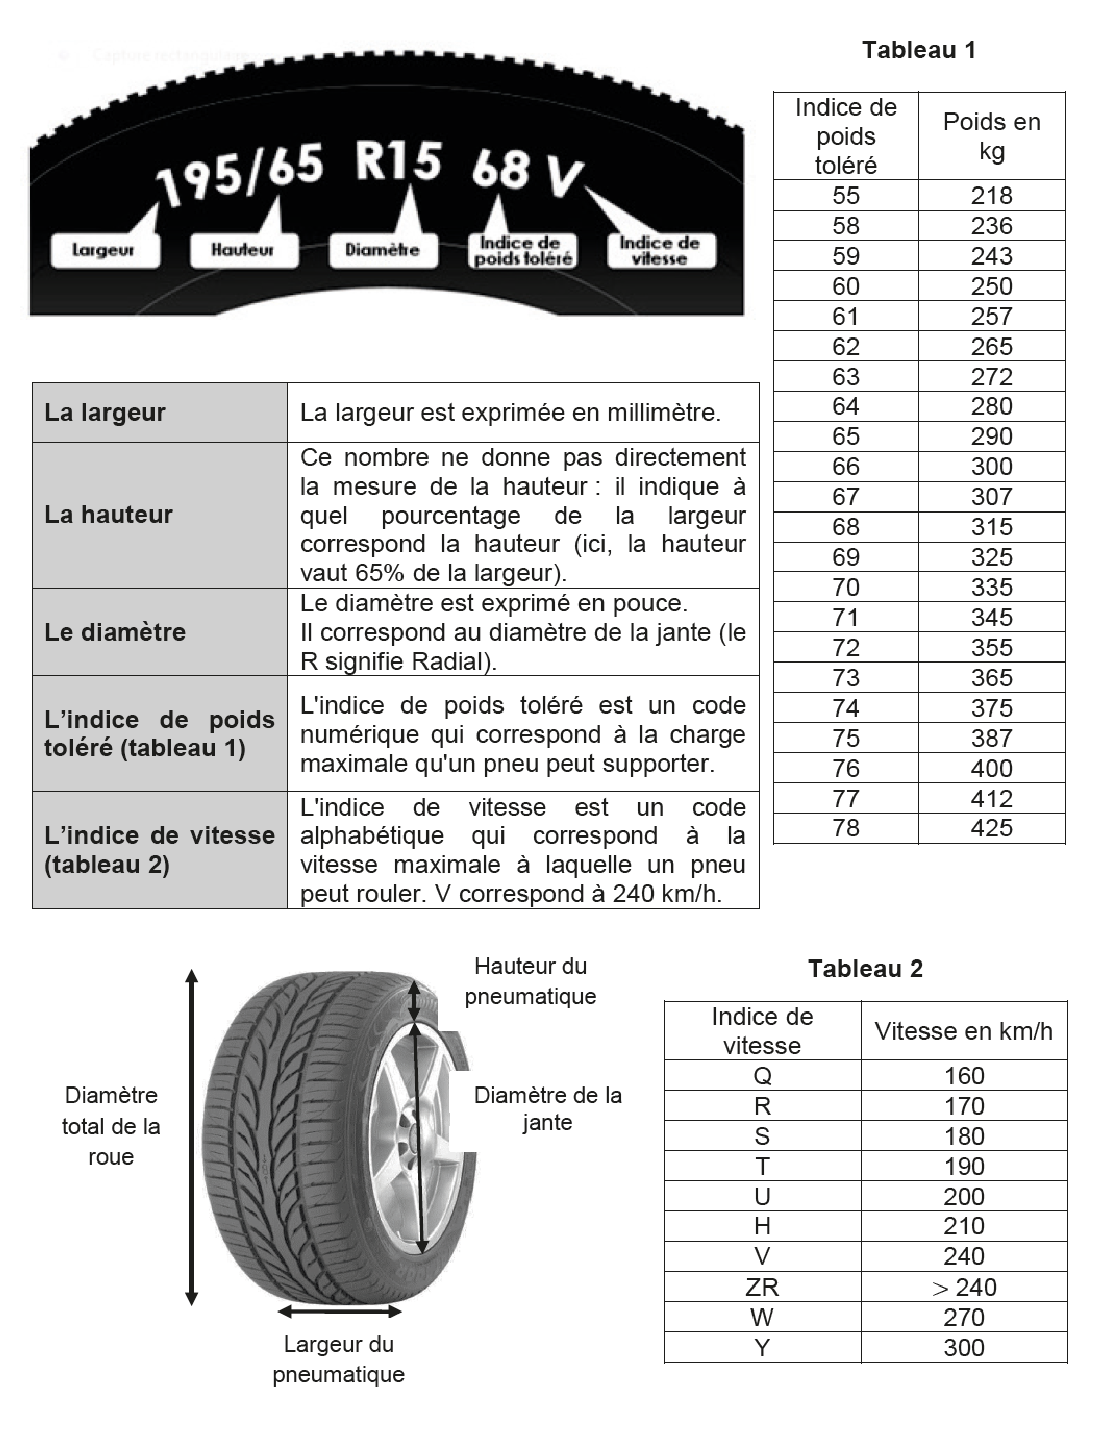
\includegraphics[width=13cm]{Grandeurs_mesures/Images/M13_ex_pneu}
   \end{center}
      \begin{enumerate}
         \item On considère un pneumatique sur lequel est inscrit \og 195/65 R15 68V \fg.
         \begin{enumerate}
            \item Sachant que 1 pouce vaut \ucm{2,54}, calculer le diamètre de la jante en centimètre.
            \item Montrer que la hauteur du pneu est \ucm{12,675}.
            \item Calculer le diamètre total de la roue en centimètre.
         \end{enumerate}
      \item On considère désormais un pneu radial pouvant supporter une charge maximale de \ukg{412} et rouler à la vitesse maximale de \ukmh{270}. Sa largeur est de \ucm{20,5}, le diamètre de sa jante est de \ucm{40,64} et son diamètre total est de \ucm{63,19}. Indiquer, sous la forme \og 195/65 R15 68V \fg, les informations qui seront inscrites sur ce pneu.
   \end{enumerate}
\end{exercice}

\begin{corrige}
\ \\ [-5mm]
   \begin{enumerate}
      \item 
         \begin{enumerate}
            \item Le diamètre est lu grâce à la côte \og R15 \fg, il s'agit donc d'une jante de diamètre 15 pouces. \\
               Or, $15\times\ucm{2,54} =\ucm{38,1}$. {\blue Le diamètre de la jante vaut \ucm{38,1}}. \\
            \item La hauteur du pneu peut-être calculée grâce à la côte \og 195/65 \fg. \\
               Donc, la hauteur du pneu vaut 65 \% de sa largeur (\umm{195}). Or, $\dfrac{65}{100}\times\umm{195} =\umm{126,75}$. \\
               {\blue La hauteur du pneu est \ucm{12,675}}. \\
            \item $\text{Diamètre de la roue} = \text{diamètre de la jante} + 2\times\text{hauteur du pneu}$ \\
               \hspace*{3.38cm} $=\ucm{38,1}+2\times\ucm{12,675}=\ucm{63,45}$. \\
               {\blue Le diamètre total de la roue est \ucm{63,45}}. \\
         \end{enumerate}
      \setcounter{enumi}{1}
      \item Les informations inscrites sur le pneu sont au nombre de cinq :
         \begin{itemize}
            \item largeur : $\ucm{20,5} = {\bf 205} \umm{}$ ;
            \item hauteur : $\text{hauteur du pneu} = \dfrac{\text{diamètre total du pneu}-\text{diamètre de la jante}}{2}$ \\ [1mm]
               \hspace*{4.7cm} $=\dfrac{\ucm{63,19}-\ucm{40,64}}{2} =\ucm{11,275}$. \\ [1mm]
               Or, une mesure de \ucm{11,275} représente un pourcentage de $\dfrac{\ucm{11,275}}{\ucm{20,5}}\times100 =\bf{55}\,\%$ par rapport à une mesure de \ucm{20,5} ;
            \item diamètre : le diamètre de la jante vaut \ucm{40,64}, qu'il faut convertir en pouce. Or, un pouce vaut \ucm{2,54} et $40,64\div2,54=16$ donc, l'inscription est {\bf R16} ;
            \item indice du poids : la charge maximale est de \ukg{412} ce qui correspond à l'indice {\bf 77} ;
            \item indice de vitesse : la vitesse maximale est de \ukmh{270} ce qui correspond à l'indice {\bf W}. \\
         \end{itemize}
         {\blue Les informations inscrites sur ce pneu sont : 205/55 R16 77 W}.
   \end{enumerate}
\end{corrige}

\bigskip


\begin{exercice}[CRPE 2018 G3] %%%7
   Une piste d'athlétisme est formée de huit couloirs. La largeur de chaque couloir est de 1,22 mètre. \\
   Chacun des neuf bords des huit couloirs est composé de deux lignes droites de 100 mètres et de deux demi-cercles. \\
   Le couloir 1 est celui le plus à l'intérieur, le 8 étant celui le plus à l'extérieur. Le bord intérieur du couloir 1 est composé de deux lignes droites de 100 mètres et de deux demi-cercles de rayon 31,83 mètres. \\
   Dans tout l’exercice on négligera la largeur des bandes de peinture délimitant les couloirs. \\
   Pour les courses de sprint (\um{100}, \um{200} ou \um{400}), il y a huit coureurs et chacun occupe un couloir. Un coureur devant rester dans son couloir tout au long de la course, on considère que la distance qu'il parcourt est celle correspondant à la ligne la plus intérieure de son couloir. 
   \begin{enumerate}
      \item On a la représentation suivante :
         \begin{center}
            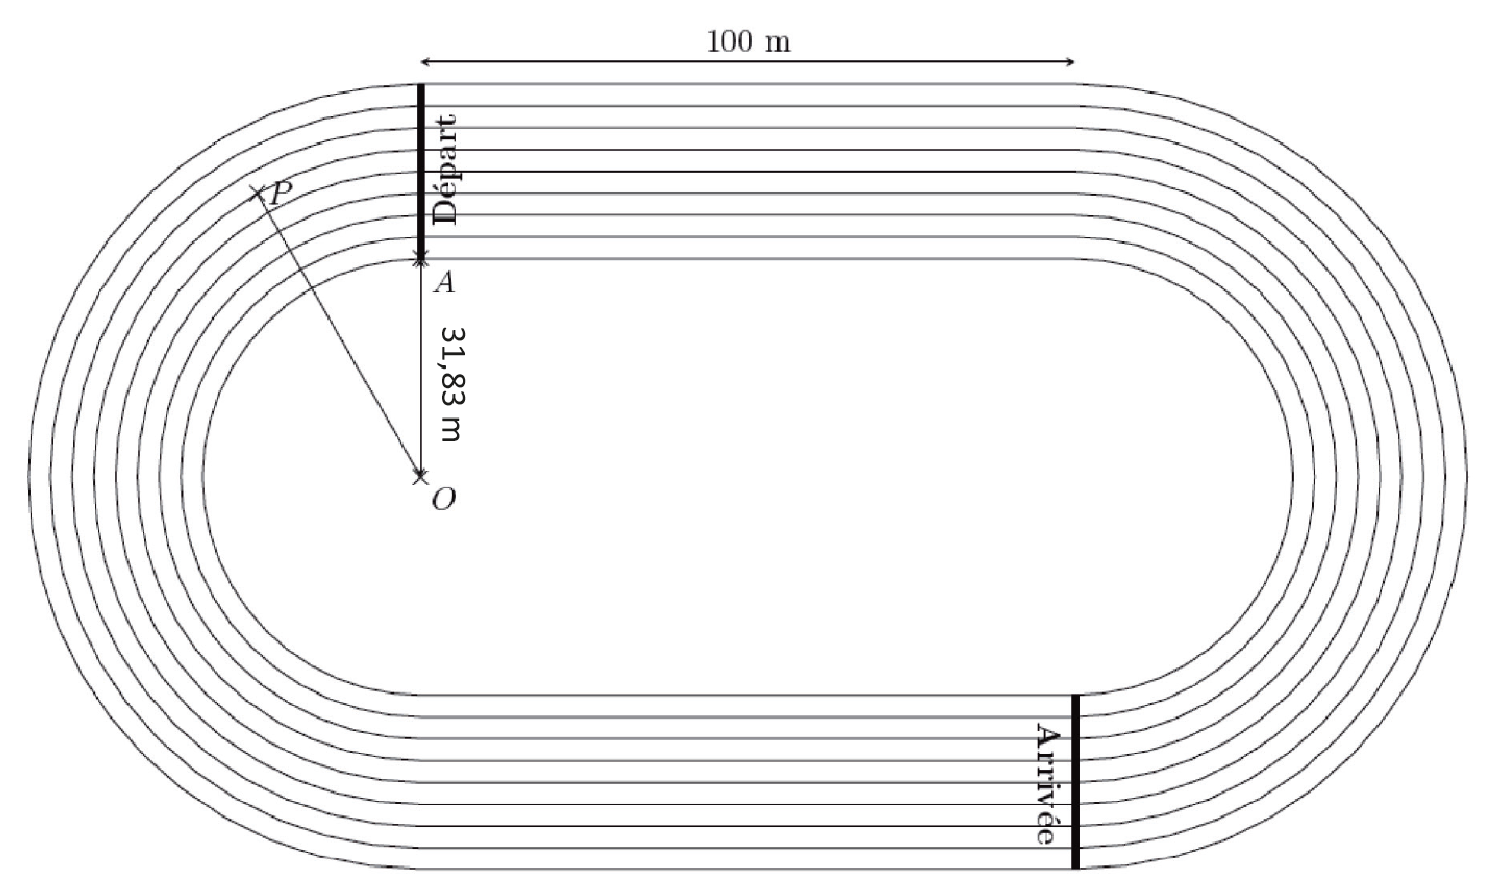
\includegraphics[width=10cm]{Grandeurs_mesures/Images/M13_ex_piste_athle}
         \end{center}
         Vérifier que la distance d’un tour de piste complet parcourue par le coureur du couloir 1 est d’environ \um{400}.
      \item Dessiner le couloir 1 (avec ses deux bords) à l’échelle 1/1200. \\
         Indiquer les calculs effectués pour réaliser la construction. \\
\hspace*{-5mm} On étudie dans les questions ci-dessous la configuration d’une course de \um{200}.
      \item Expliquer pourquoi il y a un décalage au départ d’une course de \um{200} comme sur la photographie ci-dessous : \smallskip
         \begin{center}
            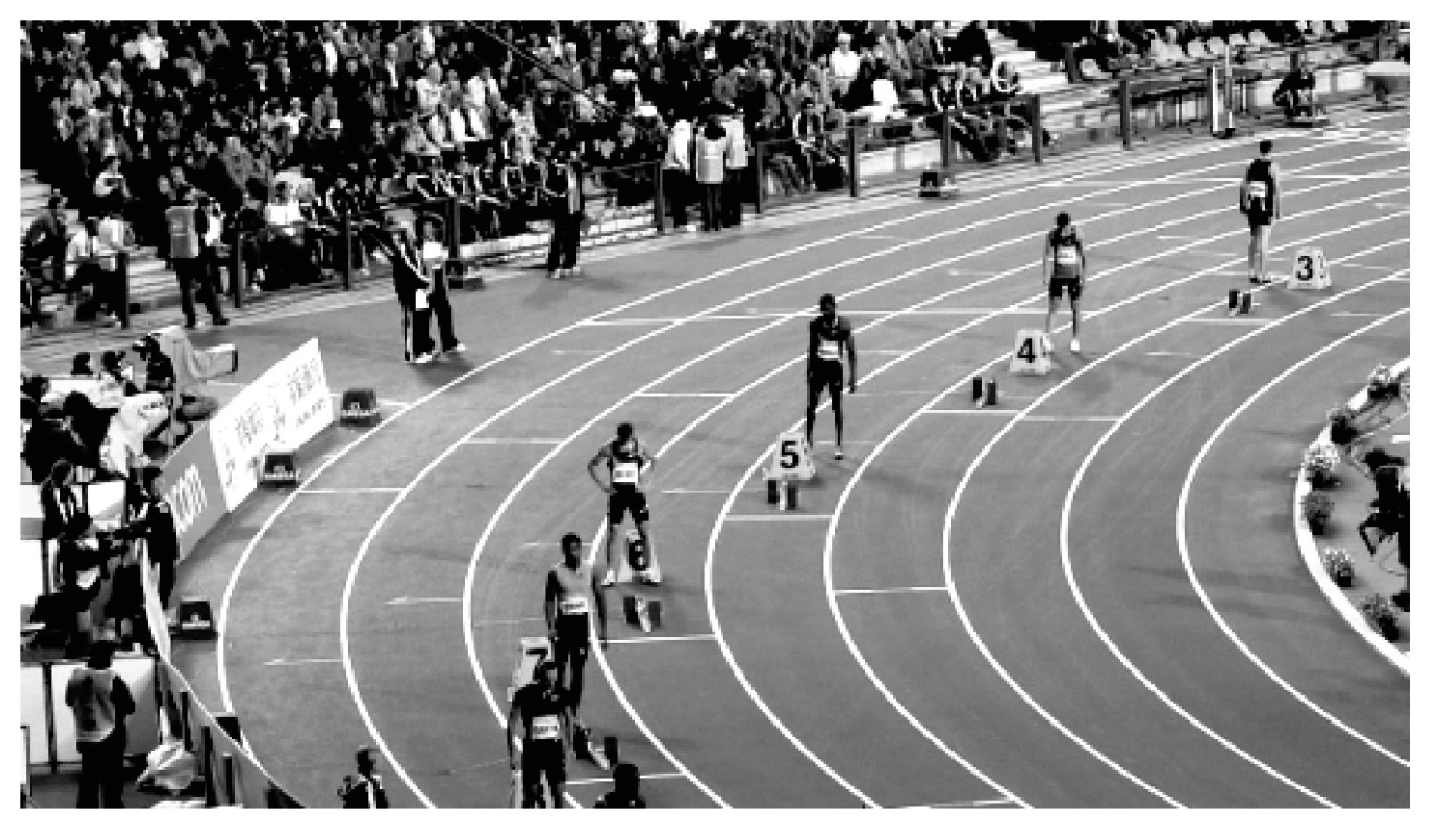
\includegraphics[width=7.2cm]{Grandeurs_mesures/Images/M13_ex_stade}
         \end{center} \smallskip
      \item Sur la représentation précédente,
         \begin{itemize}
            \item le point A correspond à la position de départ du coureur dans le couloir 1 ;
            \item le point P correspond à la position de départ du coureur dans le couloir 6. Pour ce coureur, le décalage correspond à la longueur de l'arc de cercle de centre O et qui a pour extrémités le point P et le point de la ligne 6 situé sur la ligne \og Départ \fg.
         \end{itemize}
         \vspace*{-4mm}
         \begin{enumerate}
            \item Calculer le décalage du coureur du couloir 6 au centimètre près.
            \item On peut repérer la position de départ dans le couloir par l’angle $\widehat{\text{AOP}}$ que l’on appelle $\alpha$. Cet angle dépend du numéro du couloir. Calculer la mesure de l’angle $\alpha$, au dixième de degré, pour le couloir 6. 
            \item Y a-t-il proportionnalité entre le numéro du couloir et la valeur de $\alpha$ ? Justifier.
      \end{enumerate}
   \end{enumerate}
\end{exercice}

\begin{corrige}
\ \\ [-5mm]
   \begin{enumerate}
      \item Pour effecteur un tour de piste, l'athlète doit effectuer deux lignes droites de longueur \um{100} et deux demi-tours de rayon $r =\um{31,83}$. \\
         On a alors : $L =2\times\um{100}+2\times\pi\times\um{31,83} \approx\um{399,99}$. \\
         {\blue Un tour de piste effectué en couloir 1 mesure environ \um{400}}. \\
      \item Pour dessiner le couloir 1, il faut tracer quatre segments qui correspondent aux lignes droites de mesure \um{100}.  Il faut également tracer deux demi-cercles de rayon \um{31,83} et deux demi-cercles de rayon $\um{31,83}+\um{1,22} =\um{33,05}$. \\
         À l'échelle 1/1\,200, cela correspond aux mesures suivantes : $\um{100}/1\,200 \approx\um{0,083} \approx\ucm{8,3}$ ; $\um{31,83}/1\,200 \approx\um{0,0265} \approx\ucm{2,65}$ et $\um{33,05}/1\,200 \approx\um{0,0275} \approx\ucm{2,75}$. \\
         \begin{pspicture}(-4,0)(11.5,6)
            \psline(0,0)(8.3,0)
            \psline(0,5.3)(8.3,5.3)
            \psline(0,-0.1)(8.3,-0.1)
            \psline(0,5.4)(8.3,5.4)
            \psarc(0,2.65){2.65}{90}{-90}
            \psarc(8.3,2.65){2.65}{-90}{90}
            \psarc(0,2.65){2.75}{90}{-90}
            \psarc(8.3,2.65){2.75}{-90}{90}
            \psline[linestyle=dashed]{<->}(0,2.65)(8.3,2.65)
            \psline[linestyle=dotted](0,5.3)(0,0)
            \psline[linestyle=dotted](8.3,5.3)(8.3,0)
            \rput(2.5,4){rayons : \ucm{2,65} et \ucm{2,75}}
            \rput(4.15,2.25){\ucm{8,3}}
         \end{pspicture}
   \end{enumerate}
 
\Coupe

   \begin{enumerate}
     \setcounter{enumi}{2}
      \item Sur une course de \um{200}, si les athlètes commencent tous sur la même ligne de départ perpendiculaire aux lignes droites, plus les coureurs sont éloignés du couloir 1 plus ils vont parcourir de distance puisque le rayon du demi-cercle va augmenter. Pour palier à cette injustice, il faut décaler les départs ou les arrivées. \\
         Or, pour simplifier la prise de durée et pour la beauté de l'épreuve, il est préférable que la ligne d'arrivée soit la même pour tout le monde, donc on décale les départs.
      \item 
         \begin{enumerate}
            \item Au couloir 6, si le coureur partait sur la ligne de départ matérialisée sur le schéma, il parcourrait une distance de $\pi\times\um{37,93}+\um{100}  \approx\um{219,1606}$. Il aura donc fait environ \um{19,16} en trop. \\
               {\blue Le décalage du coureur de couloir 6 est de \um{19,16}}.
            \item Un demi-tour mesure $\pi\times\um{37,93}$ et correspond à un angle de \udeg{180}. \\ [1mm]
               Donc, pour \um{19,16}, on a un angle de $\alpha =\dfrac{\um{19,16}}{37,93\,\pi\,\um{}}\times\udeg{180} \approx\udeg{28,94}$. \\ [1mm]
               {\blue La mesure de l'angle $\alpha$ est d'environ \udeg{28,9}}.
            \item Le couloir 1 correspond à une valeur de $\alpha =\udeg{0}$. Les \og zéros \fg{} ne se correspondent pas, c'est à dire que les échelles n'ont pas la même origine donc : \\
               {\blue Il n'y a pas proportionnalité entre le numéro du couloir et la valeur de $\alpha$.}
         \end{enumerate}
   \end{enumerate}
\end{corrige}

\bigskip


\begin{exercice}[CRPE 2017 G2] %%%8
   On souhaite modéliser un jardin dont l’aménagement doit être repensé. Ce jardin à la forme d'un trapèze ABCD tel que les droites (AB) et (DC) sont parallèles ; les droites (AD) et (DC) sont perpendiculaires ; AB = \um{50}, AD = \um{30} et DC = \um{70} ; E est le point du segment [DC] tel que ABED est un rectangle.
   \begin{enumerate}
      \item Représenter le jardin à l'échelle 1/1\,000\up{e}.
      \item
         \begin{enumerate}
            \item Dans un premier temps, le propriétaire désire clôturer le jardin. \\
               Calculer la longueur de clôture nécessaire sachant qu’il prévoit l’installation d’un portail de \um{3,10} de large. Donner la valeur exacte puis la valeur arrondie au mètre.
            \item Dans un deuxième temps, il partage son jardin en trois parties : \\
               \begin{minipage}{8cm}
                  \begin{itemize}
                     \item un espace potager représenté par le triangle rectangle BCE ;
                     \item un espace de plantations florales représenté par le demi-disque hachuré de diamètre [AB] ;
                     \item un espace engazonné sur le reste du jardin.
                  \end{itemize}
               \end{minipage}
               \qquad
               \begin{minipage}{8cm}
              {\psset{unit=0.7}
                \begin{pspicture}(-1.5,-0.75)(7.5,3.5)
                  \pspolygon(0,0)(5,0)(7,0)(5,3)(0,3)
                  \psline[linestyle=dashed](5,0)(5,3)
                  \rput(-0.3,-0.3){D}
                  \rput(-0.3,3.3){A}
                  \rput(5,-0.3){E}
                  \rput(7.3,-0.3){C}
                  \rput(5.3,3.3){B}
                  \pswedge[fillstyle=hlines,hatchsep=3mm](2.5,3){2.5}{180}{0}
               \end{pspicture}
            }
            \end{minipage}
            Calculer l’aire arrondie au mètre carré de chacune des trois parties du jardin.
         \end{enumerate}
   \end{enumerate}
\end{exercice}

\begin{corrige}
\ \\ [-5mm]
   \begin{enumerate}
      \item L'échelle 1/1\,000\up{e} signifie que \ucm{1000} = \um{10} dans la réalité sont représentés par \ucm{1} sur le plan. \\
    {\psset{unit=1}
      \begin{pspicture}(-3.5,-0.8)(7.5,3.8)
         \pspolygon(0,0)(5,0)(7,0)(5,3)(0,3)
         \psline[linestyle=dashed](5,0)(5,3)
         \psframe(0,0)(0.3,0.3)
         \psframe(0,3)(0.3,2.7)
         \psframe(5,0)(5.3,0.3)
         \rput(-0.3,-0.3){D}
         \rput(-0.3,3.3){A}
         \rput(5,-0.3){E}
         \rput(7.3,-0.3){C}
         \rput(5.3,3.3){B}
      \end{pspicture}
   }
   \item 
      \begin{enumerate}
         \item Dans le trapèze ABCD, calculons BC. Le triangle BEC est rectangle en E, on utilise le théorème de Pythagore avec des mesures de longueur en mètre. \\
            BC$^2$ = BE$^2$ + EC$^2 \iff \text{BC}^2 = 30^2+20^2 =1\,300 \iff \text{BC} =10\sqrt{13}$. \\
            Le périmètre du jardin vaut alors : AB + BC + CD + DA = $\um{50}+10\sqrt{13}\,\um{}+\um{70}+\um{30} =(150+10\sqrt{13})\,\um{}$. \\
            À ce périmètre, il faut enlever la largeur du portail, donc, {\blue la longueur de la clôture est de $(146,90+10\sqrt{13})\,\um{} \approx\um{183}$}
         \item
            \begin{itemize}
               \item Aire de potager : $\mathcal{A}_p =\dfrac{\text{EC}\times\text{EB}}{2} =\dfrac{\um{20}\times\um{30}}{2} =$ {\blue $\umq{300}$}.
               \item Aire des plantations florales : $\mathcal{A}_f =\dfrac12\times\pi\left(\dfrac{\text{AB}}{2}\right)^2=\dfrac12\times\pi\left(\dfrac{\um{50}}{2}\right)^2 =\dfrac{625}{2}\pi\,\umq{} \approx$ {\blue $\umq{982}$}. \smallskip
               \item Aire du gazon : $\mathcal{A}_g =\text{DE}\times\text{DA}-\mathcal{A}_f =\um{50}\times\um{30}-\dfrac{625}{2}\pi\,\umq{} =\umq{1500}-\dfrac{625}{2}\pi\,\umq{} \approx $ {\blue $\umq{518}$}.
            \end{itemize}
         \end{enumerate}
   \end{enumerate}
\end{corrige}

\bigskip


\begin{exercice}[CRPE 2021 G4]
   {\it Dans ce problème, les figures qui sont dessinées ne sont pas représentées en vraie grandeur.}
   \begin{enumerate}
      \item On souhaite partager un carré $ABCD$ de \ucm{10} de côté en trois parties comme indiqué sur la {\it figure 1}. \\
         $L$ est un point du segment $[BC]$ et $M$ est le point du segment $[CD]$ tel que $DM = BL$. On note $x$ la longueur, en centimètre, du segment $[BL]$. Les aires sont exprimées en \ucmq{}.
         \begin{enumerate}
            \item Expliquer pourquoi $0\leq x\leq10$.
           \item Vérifier que si $x =2$, alors l’aire du quadrilatère grisé $AMCL$ est égale à \ucmq{80}.
            \item Calculer l’aire du quadrilatère grisé $AMCL$ si $x =\dfrac35$. \smallskip
            \item Montrer que l’aire du quadrilatère grisé $AMCL$ en fonction de $x$ est égale à $100-10x$.
            \item Déterminer $x$ pour que les trois parties aient la même aire.
         \end{enumerate}
      \item Le triangle hachuré a été supprimé pour obtenir trois triangles $ADM, AML$ et $ALB$ de la {\it figure 2}.
         \begin{enumerate}
            \item Vérifier que si $x =2$, alors l’aire du triangle hachuré $MCL$ est égale à \ucmq{32}.
            \item Exprimer l’aire, en centimètre carré, de la partie hachurée $MCL$ en fonction de $x$.
            \item Montrer que l’aire du triangle grisé $AML$ est égale à $50-\dfrac{x^2}{2}$.
         \end{enumerate}
   \end{enumerate}
   \begin{center}
      \begin{pspicture}(0,-1)(6,4.3)
         \pstGeonode[PosAngle={-135,-45,45,135,-90,0},PointSymbol=none](0,0){D}(4,0){C}(4,4){B}(0,4){A}(2.5,0){M}(4,1.5){L}
         \psframe(D)(B)
         \pspolygon[fillstyle=solid,fillcolor=lightgray](A)(M)(C)(L)
         \pstLabelAB*[linestyle=dashed,arrows=<->,offset=-7mm]{D}{M}{$x$}
         \pstLabelAB*[linestyle=dashed,arrows=<->,offset=6mm]{B}{L}{$x$}
         \rput(2,-1.4){\small\it figure1}
      \end{pspicture}
      \quad
      \begin{pspicture}(-1,-1)(5,4.3)
         \pstGeonode[PosAngle={-135,-45,45,135,-90,0},PointSymbol=none](0,0){D}(4,0){C}(4,4){B}(0,4){A}(2.5,0){M}(4,1.5){L}
         \psframe(D)(B)
         \pspolygon[fillstyle=solid,fillcolor=lightgray](A)(M)(L)
         \pspolygon[fillstyle=vlines](C)(M)(L)
         \pstLabelAB*[linestyle=dashed,arrows=<->,offset=-7mm]{D}{M}{$x$}
         \pstLabelAB*[linestyle=dashed,arrows=<->,offset=6mm]{B}{L}{$x$}
         \rput(2,-1.4){\small\it figure2}
      \end{pspicture}
   \end{center}
\end{exercice}

\begin{corrige}
\ \\ [-5mm]
   \begin{enumerate}
      \item 
         \begin{enumerate}
            \item $L$ appartient au segment $[BC]$ de mesure \ucm{10} donc, {\blue $0\leq x\leq10$}. \smallskip
           \item $\mathcal{A}_{ABCD} =AB\times AD =(\ucm{10})^2 =\ucmq{100}$. \\ [1mm]
              Si $x =2$, alors $\mathcal{A}_{ADM} =\mathcal{A}_{ABL} =\dfrac{AD\times DM}{2} =\dfrac{\ucm{10}\times\ucm{2}}{2} =\ucmq{10}$. \\ [1mm]
              On a alors $\mathcal{A}_{AMCL} =\mathcal{A}_{ABCD}-\mathcal{A}_{ADM}-\mathcal{A}_{ABL} =\ucmq{100}-\ucmq{10}-\ucmq{10} =\ucmq{80}$. \\ [1mm]
              {\blue Si $x =2$, alors l’aire de $AMCL$ est égale à \ucmq{80}}.
            \item Si $x =\dfrac35$, alors $\mathcal{A}_{ADM} =\mathcal{A}_{ABL} =\dfrac{\ucm{10}\times\dfrac35\ucm{}}{2} =\dfrac{\ucmq{6}}{2} =\ucmq{3}$. \\ [1mm]
              On a alors $\mathcal{A}_{AMCL} =\mathcal{A}_{ABCD}-\mathcal{A}_{ADM}-\mathcal{A}_{ABL} =\ucmq{100}-\ucmq{3}-\ucmq{3} =\ucmq{94}$. \\ [1mm]
              {\blue Si $x =\dfrac35$, alors l’aire de$AMCL$ est égale à \ucmq{94}}. \smallskip
            \item $\mathcal{A}_{ABCD} =100$ et $\mathcal{A}_{ADM} =\mathcal{A}_{ABL} =\dfrac{10\times x}{2} =5x$. \\ [1mm]
              On a alors $\mathcal{A}_{AMCL} =\mathcal{A}_{ABCD}-\mathcal{A}_{ADM}-\mathcal{A}_{ABL} =100-5x-5x ={\blue 100-10x}$.
            \item Les trois parties ont la même aire si $\mathcal{A}_{ADM} =\mathcal{A}_{AMCL} =\mathcal{A}_{ABL}$ \\ [1mm]
               Soit $5x =100-10x \iff 15x =100 \iff x =\dfrac{100}{15} =\dfrac{20}{3}$. \\ [1mm]
               Cette valeur est bien dans l'intervalle $[0;10]$, on peut affirmer que {\blue $x =\dfrac{20}{3}$ est la valeur recherchée}.
         \end{enumerate}
      \setcounter{enumi}{1}
      \item 
         \begin{enumerate}
            \item Si $x =2$, alors $MC =CL =\ucm{10} -\ucm{2} =\ucm{8}$. \\ [1mm]
            D'où : $\mathcal{A}_{MCL} =\dfrac{MC\times CL}{2} =\dfrac{\ucm{8}\times\ucm{8}}{2} =\ucmq{32}$. \\ [1mm]
              {\blue Si $x =2$, alors l’aire de$MCL$ est égale à \ucmq{32}}. \smallskip
            \item ${\blue \mathcal{A}_{MCL}} =\dfrac{(10-x)\times(10-x)}{2} {\blue =\dfrac{(10-x)^2}{2}}$. \\
            \item $\mathcal{A}_{AML} =\mathcal{A}_{AMCL}-\mathcal{A}_{MCL} =(100-10x)-\dfrac{(10-x)^2}{2}$ \\ [1mm]
               \hspace*{4.2cm} $=100-10x-\dfrac{100-20x+x^2}{2}$  \\ [1mm]
               \hspace*{4.2cm} $=100-10x-50+10x-\dfrac{x^2}{2}$ \\ [1mm]
               Soit : {\blue $\mathcal{A}_{AML} =50-\dfrac{x^2}{2}$}.
         \end{enumerate}
   \end{enumerate}
\end{corrige}

\bigskip


\begin{exercice}[CRPE 2022 - Sujet 0] %%%10
   Alice veut réaliser une activité avec ses élèves de petite section de maternelle. \\
   Elle a besoin de découper 30 disques de \ucm{14} de rayon dans des feuilles de dimensions $\ucm{120}\times\ucm{80}$, c’est-à-dire de \ucm{120} de longueur sur \ucm{80} de largeur. \\
   Elle aimerait les dessiner en occupant l’espace de chaque feuille en commençant en haut à gauche puis en continuant comme dans la figure ci-dessous (qui n'est pas à l'échelle).
   \begin{center}
      \begin{pspicture}(-0.5,-1)(8,3)
         \psframe(-0.5,-1)(8,3)
         \multido{\r=0+1}{8}{\pscircle(\r,2.5){0.5}}
         \multido{\r=0+1}{3}{\pscircle(\r,1.5){0.5}}
         \rput(4,1.5){\dots}
      \end{pspicture}
   \end{center}
   \begin{enumerate}
      \item Calculer l’aire de la feuille, en \ucmq{}.
      \item
         \begin{enumerate}
            \item Expliquer pourquoi Alice peut tracer au maximum 4 disques dans la longueur de la feuille.
            \item En déduire le nombre maximum de disques qu’elle pourra tracer dans cette feuille.
            \item Combien faut-il au minimum de feuilles pour dessiner les 30 disques ?
         \end{enumerate}
      \item Représenter à l'échelle 1/8 une feuille de dimensions $\ucm{120}\times\ucm{80}$ avec les disques qu'elle peut contenir.
      \item Calculer l’aire exacte d’un disque puis donner la valeur arrondie au centimètre carré près. \\
      \hspace*{-5mm} Dans la suite du problème, on considèrera que l’aire d’un disque est de \ucmq{616}.
      \item
         \begin{enumerate}
            \item Quelle est l’aire de papier non utilisé si Alice découpe 8 disques dans une feuille ? \\
              Quelle proportion, exprimée en pourcentage et arrondie à l’unité de pourcentage, de l’aire totale de la feuille cela représente-t-il ?
           \item Quelle est l’aire de papier non utilisé après avoir découpé 30 disques ? \\
              Quelle proportion, exprimée en pourcentage et arrondie à l’unité de pourcentage, de l’aire totale des feuilles utilisées cela représente-t-il ?
         \end{enumerate}
      \item Pour limiter le gaspillage de papier, Alice veut choisir le format qui permettra d’obtenir le moins de chutes (en \ucmq{}) tout en gardant la même disposition que précédemment. \\
         Elle a le choix entre plusieurs formats proposés par un fournisseur : \smallskip
         \begin{center}
            {\hautab{1.3}
            \begin{ltableau}{0.6\linewidth}{2}
               \hline
               Nom & Dimensions \\
               \hline
               Raisin & $\ucm{65}\times\ucm{50}$ \\
               \hline
               Jésus & $\ucm{76}\times\ucm{56}$ \\
               \hline
               Impérial & $\ucm{80}\times\ucm{60}$ \\
               \hline
               Grand Aigle & $\ucm{105}\times\ucm{75}$ \\
               \hline
               Grand Monde & $\ucm{120}\times\ucm{80}$ \\
               \hline           
            \end{ltableau}
         }
         \end{center}
         Pour obtenir les 30 disques, le format Grand Aigle permet-il d’obtenir moins de chutes (en \ucmq{}) que le format Grand Monde ? Justifier la réponse.
   \end{enumerate}
\end{exercice}

\begin{corrige}
\ \\ [-5mm]
   \begin{enumerate}
      \item L'aire de la feuille vaut $\ucm{120}\times\ucm{80} ={\blue \ucmq{9600}}$.
      \item 
         \begin{enumerate}
            \item Le rayon du disque vaut \ucm{14}, donc son diamètre vaut \ucm{28}. \\
               Or, $4\times\ucm{28} =\ucm{112}$ et $5\times\ucm{28} =\ucm{140}$. La longueur de la feuille étant de \ucm{120}, {\blue Alice peut mettre au maximum quatre disques dans la longueur de la feuille}.
            \item La largeur de la feuille mesure \ucm{80}. Or, $2\times\ucm{28} =\ucm{56}$ et $3\times\ucm{28} =\ucm{84}$. Alice peut mettre au maximum deux disques dans la largeur de la feuille puisqu'elle mesure \ucm{80}. \\
               Si l'on considère la configuration de la figure (qui n'est pas optimale), on en déduit qu'{\blue Alice peut tracer au maximum huit disques sur sa feuille} ($2\times4 =8$).
            \item Alice peut tracer huit disques par feuilles, et $4\times8\text{ disques} =32\text{ disques}$ alors que $3\times8\text{ disques} =24\text{ disques}$. Donc, {\blue il faudra au minimum quatre feuilles pour dessiner les 30 disques}.
         \end{enumerate}
   \end{enumerate}
   
\Coupe
 
    \begin{enumerate}
         \setcounter{enumi}{2}
         \item À l'échelle 1/8, les dimensions respectives de \ucm{120}, \ucm{80} et \ucm{14} sont représentées par des dimensions de $\ucm{120}\div8 =\ucm{15}, \ucm{80}\div8 =\ucm{10}$ et $\ucm{14}\div8 =\ucm{1,75}$. \\
         \begin{pspicture}(-0.5,-0.25)(15,10.5)
            \psframe(0,0)(15,10)
            \multido{\r=1.75+3.5}{4}{\pscircle(\r,8.25){1.75}}
            \multido{\r=1.75+3.5}{4}{\pscircle(\r,4.75){1.75}}
         \end{pspicture}
      \item $\mathcal{A}_{\text{disque}} =\pi\times r^2 =\pi\times(\ucm{14})^2 =196\pi\,\ucmq{} \approx\ucmq{615,75}$. \\
         {\blue L'aire d'un disque vaut $196\,\pi\;\ucmq{}$, soit environ \ucmq{616}}.
      \item
         \begin{enumerate}
            \item Aire utilisée pour tracer les disques : $8\times\ucmq{616} =\ucmq{4928}$. \\
               Aire non utilisée : $\ucmq{9600}-\ucmq{4928} =\ucmq{4672}$. \\
               {\blue L'aire non utilisée pour découper les huit disques est de \ucmq{4672}}. \\
              $\dfrac{\ucmq{4972}}{\ucmq{9600}}\times100 \approx48,67$. Donc, {\blue la quantité de feuille non utilisée représente une proportion d'environ 49\,\%}. \medskip
           \item Pour les 30 disques, il faut 3 feuilles avec 8 disques et une feuille avec 6 disques. \\
           Le papier non utilisé correspond donc à $3\times\ucmq{4672}+\ucmq{9600}-6\times\ucmq{616} =\ucmq{19920}$. \\
              {\blue L’aire de papier non utilisé après avoir découpé 30 disques est de \ucmq{19920}}. \\
              $\dfrac{\ucmq{19920}}{4\times\ucmq{9600}}\times100 \approx51,875$. \\ [2mm]
              Donc, {\blue L’aire de papier non utilisé après avoir découpé 30 disques représente une proportion d'environ 52\,\%}.
         \end{enumerate}
      \setcounter{enumi}{5}
      \item On a $105 =3\times28+21$ et $75 =2\times28+19$ donc, le format Grand Aigle permet de tracer trois disques dans la longueur et deux dans la largeur, soit six disques par feuille. \\
         De plus, $30 =6\times5$ donc, il faudra cinq feuilles, remplie chacune de six disques. \\
         Pour une feuille, le gaspillage sera de $\ucm{105}\times\ucm{75}-6\times\ucmq{616} =\ucmq{7875}-\ucm{3696} =\ucm{4179}$. \\
         Soit pour cinq feuilles : $5\times\ucm{4179} =\ucm{20895}$. \\
         Par conséquent, {\blue le format Grand Aigle ne permet pas d'obtenir moins de chutes que le format Grand Monde}.
   \end{enumerate}
\end{corrige}


%\begin{exercice}[CRPE 2015 G3]
%   Un professeur souhaite proposer aux élèves de fabriquer des figures comme la {\it Figure 1}, par découpage, collage puis coloriage. Il voudrait que chacune de ces figures, qui évoque une tête, ait un \og \oe il \fg{} en forme de carré et un \og oeil \fg{} en forme de triangle équilatéral. Il dispose de feuilles cartonnées dans lesquelles il découpera des carrés. Dans ces carrés, les élèves réaliseront les différents découpages requis.
%\begin{multicols}{2} 
%\begin{center}
%{\psset{unit=0.8}
%   \begin{pspicture}(-3,-1.5)(2,1.75)
%      \pscircle(0,0){1.7}
%      \psframe[fillstyle=vlines](-0.9,0.3)(-0.2,1)
%      \pspolygon[fillstyle=vlines](0.2,0.3)(1,0.3)(0.55,1)
%      \rput(-3,0){\it\small Figure 1}
%   \end{pspicture}
%   \begin{pspicture}(-2,-1.5)(4,1.75)
%      \psframe(-1.8,-1.8)(1.8,1.8)
%      \psline[linestyle=dashed](-1.8,0)(1.8,0)
%      \psframe[fillstyle=vlines](-1.8,-1.8)(-0.2,-0.2)
%      \pspolygon[fillstyle=vlines](-0.2,-1.8)(0.8,-0.05)(1.8,-1.8)
%      \psframe[fillstyle=vlines](-1.8,1.8)(-0.2,0.2)
%      \pspolygon[fillstyle=vlines](-0.2,1.8)(0.8,0.05)(1.8,1.8)
%      \pcline{<->}(3,-1.8)(3,1.8) \nbput{7cm}
%      \rput(-3,0){\it Figure 2}
%   \end{pspicture}}
%\end{center}
%\end{multicols}
%\begin{enumerate}
%   \item
%   \begin{enumerate}
%      \item Vérifier qu'il est possible de découper dans un carré de 7 cm de côté, deux paires d'yeux formées d'un carré de côté 3 cm et d'un triangle équilatéral de côté 4 cm, dans la disposition de la {\it Figure 2}.       
%      \item Le professeur constate que les carrés et les triangles équilatéraux que les élèves auront à découper ont le même périmètre. Ont-ils la même aire ?
%   \end{enumerate}
%   \item Le professeur se demande s'il est possible de choisir d'autres dimensions pour les yeux de telle sorte qu'on puisse les découper dans des feuilles carrées de 7 cm de côté dans la disposition de la {\it Figure 2}, le carré et le triangle équilatéral ayant le même périmètre. Pour cela, il appelle $x$ le côté du carré hachuré et $y$ celui du triangle équilatéral hachuré. Expliquer pourquoi si $x$ et $y$ sont solutions du problème, ils vérifient les contraints suivantes : \\
%   $$\left\{\begin{array}{l} 4x-3y =0 \\ x+y =7 \\ 2x \leqslant7 \\ y\sqrt3 \leqslant7 \\ \end{array} \right.$$
%   En déduire la solution au problème.
%\end{enumerate}
%\end{exercice}

%\begin{corrige}
%\ \\ [-5mm]
%\begin{enumerate}
%   \item 
%   \begin{enumerate}
%      \item Sur l'un des côtés, on peut mettre côte à côte le carré et le triangle puisque la mesure du côté du carré est de 4 cm et celle du côté du triangle est de 3 cm. Or, 4 cm + 3 cm = 7 cm. \\
%      Pour l'un des côtés adjacents, la somme des mesures des côtés de deux carrés côte à côte fait 6 cm, ce qui est bien inférieur à 7 cm. \\
%      La hauteur du triangle de côté 4 cm fait $4\dfrac{\sqrt3}{2}\text{ cm} =2\sqrt{3} \ucm{} \approx 3,46$ cm, ce qui est bien inférieur à 3,5 cm. \\ [1mm]
%      On peut donc bien découper deux triangles \og l'un au dessus de l'autre \fg{}, comme sur la {\it figure 2}. \\
%      {\blue Il es possible de découper deux carrés et deux triangles comme indiqué sur la figure 2.}
%      \item Aire du carré de côté 3 cm : $\mathcal{A}_c =(3\text{ cm})^2 =9$ cm$^2$. \\
%      Aire du triangle équilatéral de côté 4 cm en cm$^2$ : $\mathcal{A}_t =\dfrac{4\times\cancel{2}\sqrt3}{\cancel{2}} =4\sqrt3 \approx6,9$. \\ [1mm]
%      {\blue Les périmètres sont égaux, mais les aires ne sont pas égales.}
%   \end{enumerate}
%   \item Si $x$ et $y$ sont solutions du problème, alors :
%      \begin{itemize}
%         \item le périmètre du carré et du triangle sont égaux, ce qui se traduit par $4\times x =3\times y$, soit {\blue $4x-3y =0$} ;
%         \item la somme des longueurs d'un côté du carré et d'un côté du triangle est de 7 cm, ce qui se traduit par {\blue $x+y =7$} ;
%         \item deux carrés doivent tenir sur un même côté du grand carré de 7 cm de côté, ce qui se traduit par {\blue $2x\leqslant7$} ;
%         \item la somme des longueurs de deux hauteurs du triangle est inférieure à 7 cm, ce qui se traduit par $\cancel{2}\times\dfrac{y\sqrt3}{\cancel{2}}\leqslant7$ {\blue $y\sqrt3\leqslant7$}.
%      \end{itemize}
%   $\begin{cases} x+y =7 \\ 4x-3y =0  \\ \end{cases}
%   \iff \begin{cases} x =7-y \\ 4(7-y)-3y =0 \end{cases}
%   \iff \begin{cases} x =7-y \\ 28-7y =0 \end{cases}
%   \iff \begin{cases} x =7-y \\ y =4 \end{cases}
%   \iff \begin{cases} x =3 \\ y =4 \end{cases}$. \\ [1mm]
%   {\blue L'unique solution du problème est le couple $(3,4)$.}
%\end{enumerate}
%\end{corrige}


%\begin{exercice}[CRPE 2018 G2]
%\begin{enumerate}
%   \item {\bf Une canette classique}. \\
%   On modélise une canette classique par un cylindre de révolution. Le volume d’un tel cylindre s’obtient en multipliant l’aire de sa base par sa hauteur. \\
%   Vérifier que le volume du cylindre, de diamètre 6,6 cm et de hauteur 9,8 cm, est supérieur à 33 cL.
%   \item {\bf Une canette slim}. \\
%   Un nouveau format de canette est apparu dernièrement sur le marché. Ces canettes allongées, dites \og slim \fg, sont plus hautes et plus fines que les précédentes, pour une même contenance. \\
%   Déterminer, au millimètre près, la plus petite hauteur possible de ce cylindre de diamètre 5,6 cm pour que la canette contienne au moins 33 cL.
%   \item {\bf Étude du lien entre le rayon de la base d’une canette de 33 cL et l’aire de son patron}. \\
%      On appelle $r$ le rayon, en centimètre, de la base du cylindre modélisant une canette de 33 cL et h sa hauteur, en centimètre.
%   \begin{enumerate}
%      \item Vérifier que $h =\dfrac{330}{\pi r^2}$. \\ [-5mm]
%      \item La figure ci-dessous représente le patron du cylindre. Celui-ci est formé de deux disques, et d’un rectangle de largeur $h$ et de longueur $L$, exprimée en centimètre. Exprimer la longueur $L$ en fonction de $r$.
%      \begin{center}
%      \begin{pspicture}(0,-2)(5,4)
%         \psframe(0,0)(4.5,2)
%         \pscircle(1.8,2.72){0.72}
%         \pscircle(1.8,-0.72){0.72}
%         \psline{<->}(4.8,0)(4.8,2)
%         \rput(5,1){$h$}
%         \psline{<->}(0,1.6)(4.5,1.6)
%         \rput(2.25,1.3){$L$}
%         \psline{<->}(1.8,2.72)(2.52,2.72)
%         \rput(2.15,2.5){$r$}
%      \end{pspicture}
%      \end{center}
%      \item Vérifier que l’aire, en centimètre carré, de la partie rectangulaire du patron est $\dfrac{660}{r}$.
%      \item Exprimer l’aire totale $\mathcal{A}$ du patron du cylindre, en centimètre carré, en fonction de $r$.
%   \end{enumerate}
%\end{enumerate}
%\end{exercice}

%\begin{corrige}
%\ \\ [-5mm]
%\begin{enumerate}
%   \item Volume de la canette classique de rayon 3,3 cm et de hauteur 9,8 cm : \\
%   $\mathcal{V}_c =\pi\times(3,3\text{ cm})^2\times9,8\text{ cm} \approx 335\text{ cm}^3 \approx0,335\text{ dm}^3 \approx0,335\text{ L} \approx33,5\text{ cL}$. \\
%   Or, 33,5 cL > 33 cL donc, {\blue le volume de cette canette est supérieur à 33 cL.}
%   \item Une contenance de 33 cL = 0,33 L correspond à un volume de 0,33 dm$^3$ = 330 cm$^3$. \\
%   Volume de la canette slim de rayon 2,8 cm et de hauteur $h$ en cm : \\
%   $\mathcal{V}_s =\pi\times(2,8\text{ cm})^2\times h\text{ cm} \geq 330\text{ cm}^3 \iff h \geq \dfrac{330\text{ cm}^3}{\pi\times7,84\text{ cm}^2} \iff h \geq 13,39\text{ cm}$. \\ [1mm]
%   {\blue Pour avoir un volume au moins égal à 33 cL, la hauteur doit être au moins égale à 13,4 cm.}
%   \item Dans toutes cette partie, les mesures de longueur sont exprimées en centimètre et les mesures d'aire en centimètre carré. \\
%   \begin{enumerate}
%      \item $\mathcal{V} =\pi\times r^2\times h =330 \iff$ {\blue $h =\dfrac{330}{\pi r^2}$.}
%      \item La longueur $L$ du rectangle correspond au périmètre du disque de rayon $r$ donc : {\blue $L =2\pi r$.}
%      \item $\mathcal{A} =L\times h =2\pi r\times\dfrac{330}{\pi r^2} =$ {\blue $\dfrac{660}{r}$.}
%      \item L'aire totale du patron est la somme de l'aire du rectangle et des deux disques : {\blue $\mathcal{A}_T =\dfrac{660}{r}+2\pi r^2$.}
%   \end{enumerate}
%\end{enumerate}
%\end{corrige}


%\begin{exercice}[Curvica\dots{} le retour !]
%\ \\ [-10mm]
%\begin{enumerate}
%   \item Déterminer les 24 formes possibles de curvica non superposables. \\
%   \curvica{\rput(1,1){a}} \curvica{\rput(1,1){b}} \curvica{\rput(1,1){c}} \curvica{\rput(1,1){d}} \\
%   \curvica{\rput(1,1){e}} \curvica{\rput(1,1){f}} \curvica{\rput(1,1){g}} \curvica{\rput(1,1){h}} \\
%   \curvica{\rput(1,1){i}} \curvica{\rput(1,1){j}} \curvica{\rput(1,1){k}} \curvica{\rput(1,1){l}} \\
%   \curvica{\rput(1,1){m}} \curvica{\rput(1,1){n}} \curvica{\rput(1,1){o}} \curvica{\rput(1,1){p}} \\
%   \curvica{\rput(1,1){q}} \curvica{\rput(1,1){r}} \curvica{\rput(1,1){s}} \curvica{\rput(1,1){t}} \\
%   \curvica{\rput(1,1){u}} \curvica{\rput(1,1){v}} \curvica{\rput(1,1){w}} \curvica{\rput(1,1){x}} \\
%   \item Classer les pièces de curvica par ordre croissant des périmètres.
%   \item Classer les pièces de curvica par ordre croissant des aires.
%\end{enumerate}
%\end{exercice}

%\begin{corrige}
%\ \\ [-5mm]
%\begin{enumerate}
%   \item Les 24 pièces différentes du curvica : \\ [1mm]
%   {\psset{unit=0.9}
%   \curvica{\rput(1,1){a} \psline(0,0)(0,2) \psline(0,2)(2,2) \psline(2,2)(2,0) \psarc(1,-2){2.24}{63.4}{116.6}}
%   \curvica{\rput(1,1){b} \psline(0,0)(0,2) \psline(0,2)(2,2) \psarc(4,1){2.24}{153.4}{-153.4} \psarc(1,2){2.24}{-116.6}{-63.4}}
%   \curvica{\rput(1,1){c} \psarc(2,1){2.24}{153.4}{-153.4} \psline(2,0)(2,2) \psline(0,2)(2,2) \psarc(1,2){2.24}{-116.6}{-63.4}}
%   \curvica{\rput(1,1){d} \psline(0,0)(0,2) \psline(2,0)(2,2) \psline(0,2)(2,2) \psline(0,0)(2,0)} \\ [1mm]
%   
%   \curvica{\rput(1,1){e} \psline(0,0)(0,2) \psline(2,0)(2,2) \psarc(1,0){2.24}{63.4}{116.6} \psarc(1,2){2.24}{-116.6}{-63.4}}
%   \curvica{\rput(1,1){f} \psline(0,0)(0,2) \psline(2,0)(2,2) \psarc(1,4){2.24}{-116.6}{-63.4} \psarc(1,2){2.24}{-116.6}{-63.4}}
%   \curvica{\rput(1,1){g} \psline(0,0)(0,2) \psline(2,0)(2,2) \psarc(1,4){2.24}{-116.6}{-63.4} \psarc(1,-2){2.24}{63.4}{116.6}}
%   \curvica{\rput(1,1){h} \psline(0,0)(0,2) \psline(2,0)(2,2) \psline(0,2)(2,2) \psarc(1,2){2.24}{-116.6}{-63.4}} \\ [1mm]
%   
%   \curvica{\rput(1,1){i} \psline(0,0)(0,2) \psarc(1,4){2.24}{-116.6}{-63.4} \psarc(4,1){2.24}{153.4}{-153.4} \psarc(1,2){2.24}{-116.6}{-63.4}} 
%   \curvica{\rput(1,1){j} \psarc(2,1){2.24}{153.4}{-153.4} \psarc(1,4){2.24}{-116.6}{-63.4} \psarc(4,1){2.24}{153.4}{-153.4} \psarc(1,-2){2.24}{63.4}{116.6}}
%   \curvica{\rput(1,1){k} \psarc(2,1){2.24}{153.4}{-153.4} \psarc(0,1){2.24}{-26.6}{26.6} \psarc(1,0){2.24}{63.4}{116.6} \psarc(1,2){2.24}{-116.6}{-63.4}}
%   \curvica{\rput(1,1){l} \psarc(-2,1){2.24}{-26.6}{26.6} \psline(2,0)(2,2) \psarc(1,4){2.24}{-116.6}{-63.4} \psarc(1,-2){2.24}{63.4}{116.6}} \\ [1mm]
%   
%   \curvica{\rput(1,1){m} \psline(0,0)(0,2) \psarc(0,1){2.24}{-26.6}{26.6} \psarc(1,4){2.24}{-116.6}{-63.4} \psarc(1,-2){2.24}{63.4}{116.6}} 
%   \curvica{\rput(1,1){n} \psarc(-2,1){2.24}{-26.6}{26.6} \psarc(4,1){2.24}{153.4}{-153.4} \psarc(1,0){2.24}{63.4}{116.6} \psarc(1,2){2.24}{-116.6}{-63.4}}
%   \curvica{\rput(1,1){o} \psarc(2,1){2.24}{153.4}{-153.4} \psarc(1,4){2.24}{-116.6}{-63.4} \psarc(4,1){2.24}{153.4}{-153.4} \psarc(1,2){2.24}{-116.6}{-63.4}}
%   \curvica{\rput(1,1){p} \psarc(2,1){2.24}{153.4}{-153.4} \psline(2,0)(2,2) \psarc(1,0){2.24}{63.4}{116.6} \psarc(1,-2){2.24}{63.4}{116.6}} \\ [1mm]
%   
%      \curvica{\rput(1,1){q} \psline(0,0)(0,2) \psarc(4,1){2.24}{153.4}{-153.4} \psarc(1,0){2.24}{63.4}{116.6} \psarc(1,2){2.24}{-116.6}{-63.4}}
%      \curvica{\rput(1,1){r} \psarc(2,1){2.24}{153.4}{-153.4} \psarc(0,1){2.24}{-26.6}{26.6} \psarc(1,4){2.24}{-116.6}{-63.4} \psarc(1,2){2.24}{-116.6}{-63.4}}
%      \curvica{\rput(1,1){s} \psarc(-2,1){2.24}{-26.6}{26.6} \psarc(1,4){2.24}{-116.6}{-63.4} \psarc(4,1){2.24}{153.4}{-153.4} \psarc(1,-2){2.24}{63.4}{116.6}}
%      \curvica{\rput(1,1){t} \psarc(2,1){2.24}{153.4}{-153.4} \psline(2,0)(2,2) \psarc(1,0){2.24}{63.4}{116.6} \psarc(1,2){2.24}{-116.6}{-63.4}} \\ [1mm]
%      
%      \curvica{\rput(1,1){u} \psline(0,0)(0,2) \psarc(1,4){2.24}{-116.6}{-63.4} \psarc(4,1){2.24}{153.4}{-153.4} \psline(0,0)(2,0)} 
%      \curvica{\rput(1,1){v} \psarc(2,1){2.24}{153.4}{-153.4} \psarc(1,4){2.24}{-116.6}{-63.4} \psarc(4,1){2.24}{153.4}{-153.4} \psline(0,0)(2,0)}
%      \curvica{\rput(1,1){w} \psarc(2,1){2.24}{153.4}{-153.4} \psarc(1,0){2.24}{63.4}{116.6} \psarc(4,1){2.24}{153.4}{-153.4} \psline(0,0)(2,0)}
%      \curvica{\rput(1,1){x} \psarc(2,1){2.24}{153.4}{-153.4} \psarc(1,4){2.24}{-116.6}{-63.4} \psline(2,0)(2,2) \psline(0,0)(2,0)}
%      } 
%   \bigskip
%   \item d < a ; h < b ; c ; e ; f ; g ; u ; x < i ; l ; m ; p ; q ; t ; v  ; w < j ; k ; n ; o ; r ; s.
%   \item s < l < g ; j ; u < a ; i ; m ; v < b ; d ; f ; n ; o ; x < h ; p ; q ; w < c ; e ; r < t ; k.
%\end{enumerate}
%\end{corrige}


%\begin{exercice}[CRPE 2005 Réunion] %%%%%%%%%%%%%%%%%%%
%   Deux terrains ont le même prix de vente.
%   \begin{itemize}
%      \item Le premier est un rectangle de largeur \um{26}. II est vendu 130 euros le mètre carré.
%      \item Le second est un trapèze qui a pour dimensions : hauteur \um{52}, grande base \um{80}, petite base \um{50}. II est vendu 110 euros le mètre carré.
%   \end{itemize}
%   Calculer la longueur du premier terrain.
%\end{exercice}
%
%\begin{corrige} 
%\begin{itemize}
%   \item Surface du second terrain en \umq{} : $\mathcal{A} =\dfrac{(\um{80}+\um{50})\times \um{52}}{2} =\umq{3380}$. \\
%   Or, $3\,380\times110 =371\,800$. Donc, le prix de vente de chaque terrain est de 371\,800 \euro.
%   \item Soit $L$ la longueur en mètre du premier terrain rectangulaire, alors on à l'équation : \\ [1mm]
%   $26\times L\times 130 =371\,000$, soit $L =\dfrac{371\,800}{26\times130} =110$. \\ [1mm]
%   {\blue Le premier terrain a une longueur de 110 mètres.}
%\end{itemize}
%\end{corrige}


%\begin{exercice}[CRPE 2007 G1] %%%%%%%%%%%%%%%%%%%
%   \ \\
%   \begin{minipage}{10cm}
%      La figure ci-contre est composée : d'un triangle isocèle ABC, rectangle en B, et de trois demi-cercles ayant ses côtés pour diamètres.
%      \begin{enumerate}
%         \item À l'aide de la règle et du compas, reproduire cette figure (laisser apparents les traits de construction).
%         \item Sachant que AC = \ucm{7}, calculer l'aire totale des surfaces grisées (au mm$^2$ près).
%      \end{enumerate}
%   \end{minipage}
%   \hspace*{1cm}
%   \begin{minipage}{7cm}
%   {\psset{unit=0.8}
%   \begin{pspicture}(-2,-2)(4,4)
%      \pswedge[fillstyle=solid,fillcolor=lightgray](2,0){2}{180}{0}
%      \pswedge[fillstyle=solid,fillcolor=lightgray](0,2){2}{90}{270}
%      \pswedge[fillstyle=solid,fillcolor=white](2,2){2.82}{135}{-45}
%      \psline(0,4)(0,0)(4,0)
%      \psframe(0,0)(0.3,0.3)
%      \rput(0,2){/\!/}
%      \rput(2,0){/\!/}
%      \rput(4.3,0){A}
%      \rput(-0.3,-0.3){B}
%      \rput(0,4.3){C}
%   \end{pspicture}}
%   \end{minipage}
%\end{exercice}

%\begin{corrige}
%\ \\ [-5mm]
%\begin{enumerate}
%   \item Il s'agit de ce que l'on appelle {\bf les lunules d'Hippocrate}, mathématicien grec (400 av. J.-C.), qui cherche à résoudre la quadrature du cercle qui consiste à construire un carré de même aire q'un cercle donné à la règle et au compas.
%   \item On appelle $T$ l'aire du triangle rectangle, $G$ l'aire du grand demi-disque de diamètre [AC] et $P$ l'aire d'un petit demi-disque de diamètre [AB], alors l'aire des surfaces grisées est égale à $T + 2P - G$. \\
%   Les longueurs sont exprimées en cm, les aires en \ucmq{}.
%   \begin{itemize}
%      \item {\blue Calcul de $T$ :} dans le triangle ABC rectangle isocèle en B, d'après le théorème de Pythagore, on a : $\text{AB}^2+\text{BC}^2 =\text{AC}^2 \iff \text{AB}^2+\text{AB}^2 =7^2 \iff 2\text{AB}^2 =49 \iff \text{AB}^2 =\dfrac{49}{2}$. \\
%      Donc, $\dfrac{\text{AB}\times \text{BC}}{2} =\dfrac{\text{AB}^2}{2} =\dfrac{49}{4}$, c'est à dire $T =\dfrac{49}{4}\ucmq{}$.
%      \item {\blue Calcul de $P$ :} l'aire d'un disque de rayon $r$ vaut $\pi r^2$, donc, \\ [1mm]
%      $P =\dfrac{\pi r^2}{2}$ avec $r^2 =\left(\dfrac{\text{AB}}{2}\right)^2 =\dfrac{\text{AB}^2}{4} =\dfrac{49}{8}$. D'où $P =\dfrac12\pi\times\dfrac{49}{8}\ucmq{} =\dfrac{49}{16}\pi\,\ucmq{}.$
%      \item {\blue Calcul de $G$ :} comme précédemment, $G =\dfrac{\pi \times\dfrac{49}{4}\ucmq{}}{2} =\dfrac{49}{8}\pi \,\ucmq{}$. \\ [1mm]
%   \end{itemize}
%   L'aire des lunules est donc de $T + 2P - G =\dfrac{49}{4}\ucmq{}+2\times\dfrac{49}{16}\pi\ucmq{}-\dfrac{49}{8}\pi\ucmq{} =\dfrac{49}{4}\ucmq{}$. \\ [1mm]
%   {\blue L'aire totale des surfaces grisées est de \ucmq{12,25}.}
%\end{enumerate}
%\end{corrige}

